%First Beamer Talk

\documentclass{beamer}

% Setup appearance:

\usetheme{Darmstadt}
%\usecolortheme{lily}
%\usefonttheme[onlylarge]{structurebold}
%\setbeamerfont*{frametitle}{size=\normalsize,series=\bfseries}
%\useinnertheme{circles}


% Standard packages

\usepackage[english]{babel}
\usepackage[latin1]{inputenc}
%\usepackage{times}
\usepackage[T1]{fontenc}
\usepackage{multirow}
\usepackage{capt-of}
\usepackage{graphicx}
\usepackage{array}
\usepackage{tikz}

\setbeamertemplate{blocks}[rounded] [shadow=false]

% Some optional colors. Change or add as you see fit.
%---------------------------------------------------
 \definecolor{ualbertagreen}{HTML}{007C41}
\definecolor{ualbertagold}{HTML}{FFDB05}


% Some optional color adjustments to Beamer. Change as you see fit.
%------------------------------------------------------------------
\setbeamercolor{frametitle}{fg=ualbertagreen,bg=white}
\setbeamercolor{title}{fg=ualbertagreen,bg=white}
\setbeamercolor{author}{fg=ualbertagreen,bg=white}
\setbeamercolor{date}{fg=ualbertagreen,bg=white}
\setbeamercolor{affiliation}{fg=ualbertagreen,bg=white}
\setbeamercolor{institute}{fg=ualbertagreen,bg=white}
\setbeamercolor{local structure}{fg=ualbertagreen}
\setbeamercolor{section in toc}{fg=ualbertagreen,bg=white}
% \setbeamercolor{subsection in toc}{fg=ualbertagreen,bg=white}
\setbeamercolor{footline}{fg=ualbertagreen!50, bg=white}
\setbeamercolor{block title}{fg=ualbertagreen,bg=white}
\setbeamercolor{upper separation line head}{bg=ualbertagreen}
\setbeamercolor{lower separation line head}{bg=ualbertagold}
\setbeamercolor{middle separation line head}{bg=ualbertagold}
\setbeamercolor{frametitle}{fg=ualbertagreen,bg=white}

\setbeamercolor{section in head/foot}{bg=white,fg=ualbertagreen}
\setbeamercolor{author in head/foot}{bg=white,fg=ualbertagreen}
\setbeamercolor{date in head/foot}{bg=white,,fg=ualbertagreen}
\setbeamercolor{title in head/foot}{bg=white,fg=ualbertagreen}

\setbeamercolor{headline}{bg=white,fg=ualbertagreen}




\setbeamercolor{middle separation line head}{bg=ualbertagreen}
\setbeamercolor{alerted text}{fg=red}
\setbeamercolor{example text}{fg=black}
\setbeamercolor{structure}{fg=black}

% Various cosmetic things, though I must confess I forget what exactly these do and why I included them.
%-------------------------------------------------------------------------------------------------------
\setbeamercolor{structure}{fg=ualbertagreen}


\setbeamercolor{local structure}{parent=structure}
\setbeamercolor{item projected}{parent=item,use=item,fg=ualbertagreen,bg=white}
\setbeamercolor{enumerate item}{parent=item}

\setbeamertemplate{title page}{%
  \vbox{}
%  \vfill
    \vspace{0cm}% NEW
  \begingroup
    \centering
    \begin{beamercolorbox}[sep=8pt,center]{title}
      \usebeamerfont{title}\inserttitle\par%
      \ifx\insertsubtitle\@empty%
      \else%
        \vskip0.05em%
        {\usebeamerfont{subtitle}\usebeamercolor[fg]{subtitle}\insertsubtitle\par}%
      \fi%
    \end{beamercolorbox}%
    \vskip1em\par
    \begin{beamercolorbox}[sep=8pt,center]{author}
      \usebeamerfont{author}\insertauthor
    \end{beamercolorbox}
    \begin{beamercolorbox}[sep=8pt,center]{institute}
      \usebeamerfont{institute}\insertinstitute
    \end{beamercolorbox}
    \vspace{0.5cm}% NEW
    \begin{beamercolorbox}[sep=8pt,center]{date}
      \usebeamerfont{date}\insertdate
    \end{beamercolorbox}\vskip0.05em
%    {\usebeamercolor[fg]{titlegraphic}\inserttitlegraphic\par}
  \endgroup
%  \vfill
}


\logo{
   \tikz [remember picture,overlay]
    \node[yshift=.3cm,xshift=1.5cm] at (current page.south west)
        %or: (current page.center)
        {
\includegraphics[width=1in]{UA-COLOUR.png}};
%
\includegraphics[height=0.8cm]{UA-ASB-COLOUR.png}\vspace{220pt}
}




\setbeamertemplate{headline}{%
\leavevmode%
  \hbox{%
    \begin{beamercolorbox}[wd=\paperwidth,ht=5ex,dp=1.825ex]{white}%
    \usebeamerfont{headline}\hskip6pt\inserttitle\par%
    \insertsectionnavigationhorizontal{\paperwidth}{}{\hskip0pt plus1filll}
    \end{beamercolorbox}%
  }
}

\setbeamertemplate{sidebar right}{}


\logo{
   \tikz [remember picture,overlay]
    \node[yshift=.3cm,xshift=1.5cm] at (current page.south west)
        %or: (current page.center)
        {
\includegraphics[width=1in]{UA-COLOUR.png}};
%
\includegraphics[height=0.8cm]{UA-ASB-COLOUR.png}\vspace{220pt}
}




%\setbeamertemplate{footline}{%
%\hfill\usebeamertemplate***{navigation symbols}
%\hspace{1cm}\insertframenumber{}/\inserttotalframenumber}
\defbeamertemplate*{footline}{my footline}{%
    \ifnum\insertpagenumber=1
        \Tiny{%
            \hfill%
		\vspace*{1pt}%
            %\insertframenumber/\inserttotalframenumber \hspace*{0.1cm}%
            \newline%
            \color{ualbertagold}{\rule{\paperwidth}{0.4mm}}\newline%
            \color{ualbertagold}{\rule{\paperwidth}{.4mm}}%
        }
%    \hbox{%
%        \begin{beamercolorbox}[wd=\paperwidth,ht=.8ex,dp=1ex,center]{}%
%      % empty environment to raise height
%        \end{beamercolorbox}%
%    %}%
    %\vskip0pt%
    %no page number on the first page
    %    \Tiny{%
    %        \hfill%
   % 		\vspace*{1pt}%
    %        \color{ualbertagold}{\rule{\paperwidth}{0.4mm}}\newline%
    %        \color{ualbertagold}{\rule{\paperwidth}{.4mm}}%
%        }%
  \else%
        \Tiny{%
            \hfill%
		\vspace*{1pt}%
            \insertframenumber/\inserttotalframenumber \hspace*{0.1cm}%
            \newline%
            \color{ualbertagold}{\rule{\paperwidth}{0.4mm}}\newline%
            \color{ualbertagold}{\rule{\paperwidth}{.4mm}}%
        }%
    \fi%
}









\renewcommand{\(}{\begin{columns}}
\renewcommand{\)}{\end{columns}}
\newcommand{\<}[1]{\begin{column}{#1}}
\renewcommand{\>}{\end{column}}
%%%%%%%%%%%%%%%%%%%%%%%%%%%%%%%%%%%%%%%%%%%%%%%%%%





% Author, Title, etc.

\title[Electricity Slide Pack]
{%
  Electricity Markets%
}

\author[Leach]
{
  Andrew~Leach
}

\institute[2017]
{
  Department of Economics and Faculty of Law, University of Alberta
 }

\date[5/28/2017]
{\today}


\newcommand{\degC}{$^o$C$\,$}
\newcommand{\co}{$\text{CO}_{2}\,$}
\newcommand{\tx}{$G_{2\times\text{CO}_2}$}
\newcommand{\Real}{\mathbb R}



% The main document


\begin{document}

\begin{frame}
   \tikz [remember picture,overlay]
    \node[yshift=-0.5cm,xshift=-1.7cm] at (current page.north east)
        %or: (current page.center)
        %\node[yshift=-0.75cm,xshift=4.5cm] at (current page.north west)
        %{
\includegraphics[width=3in]{UA-ASB-COLOUR.png}};
        {
\includegraphics[width=1in]{UA-COLOUR.png}}; \vspace{1cm}
   \titlepage
   \vfill
\end{frame}



\section{Introduction}




\begin{frame}{Why should you care about electricity?}
\begin{itemize}
\setlength\itemsep{.5em}
\item Price volatility:
\begin{itemize}
\setlength\itemsep{.5em}
    \item Electricity prices are an order of magnitude more volatile than oil or gas prices
    \item
         Both supply and demand in Alberta affect us more than global or regional supplies and demands in oil and gas markets
\end{itemize}
\item New technology:
\begin{itemize}
\setlength\itemsep{.5em}
\item Electricity is, arguably, changing faster than any other energy market
\item Alberta's electricity market is entering a period of market- and regulatory-driven transition
\end{itemize}
\item Economics 101 in action
\begin{itemize}
\setlength\itemsep{.5em}
\item Nowhere else will you see supply and demand curves actually mapped out in real time determining prices as clearly as in Alberta's power market
\end{itemize}

\end{itemize}

\vfill
\end{frame}

\begin{frame}{Price Volatility}
   \tikz [remember picture,overlay]
    \node[yshift=-.5cm,xshift=0cm] at (current page.center)
        {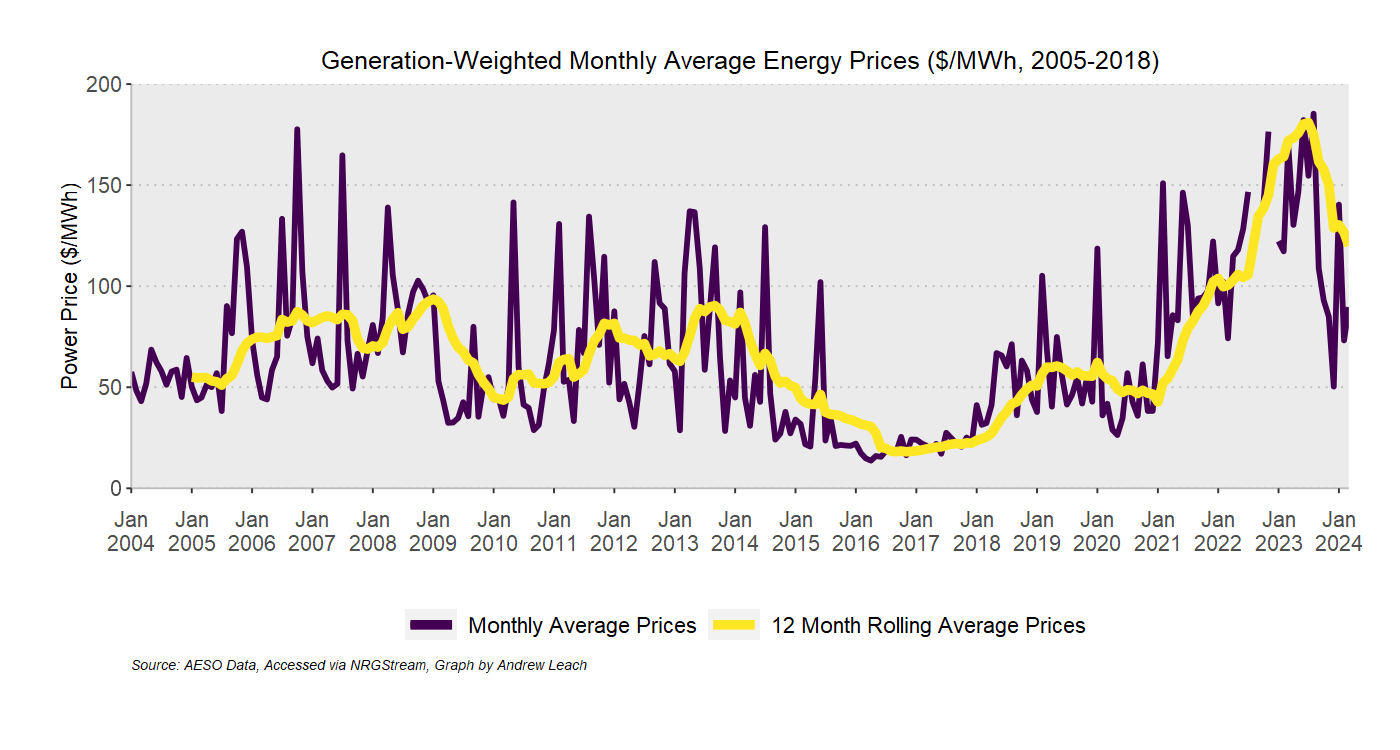
\includegraphics[width=.9\paperwidth]{../images/monthly_prices.png}}; \vspace{1cm}
   \vfill
\end{frame}


\begin{frame}{Price Volatility}
   \tikz [remember picture,overlay]
    \node[yshift=-.5cm,xshift=0cm] at (current page.center)
        {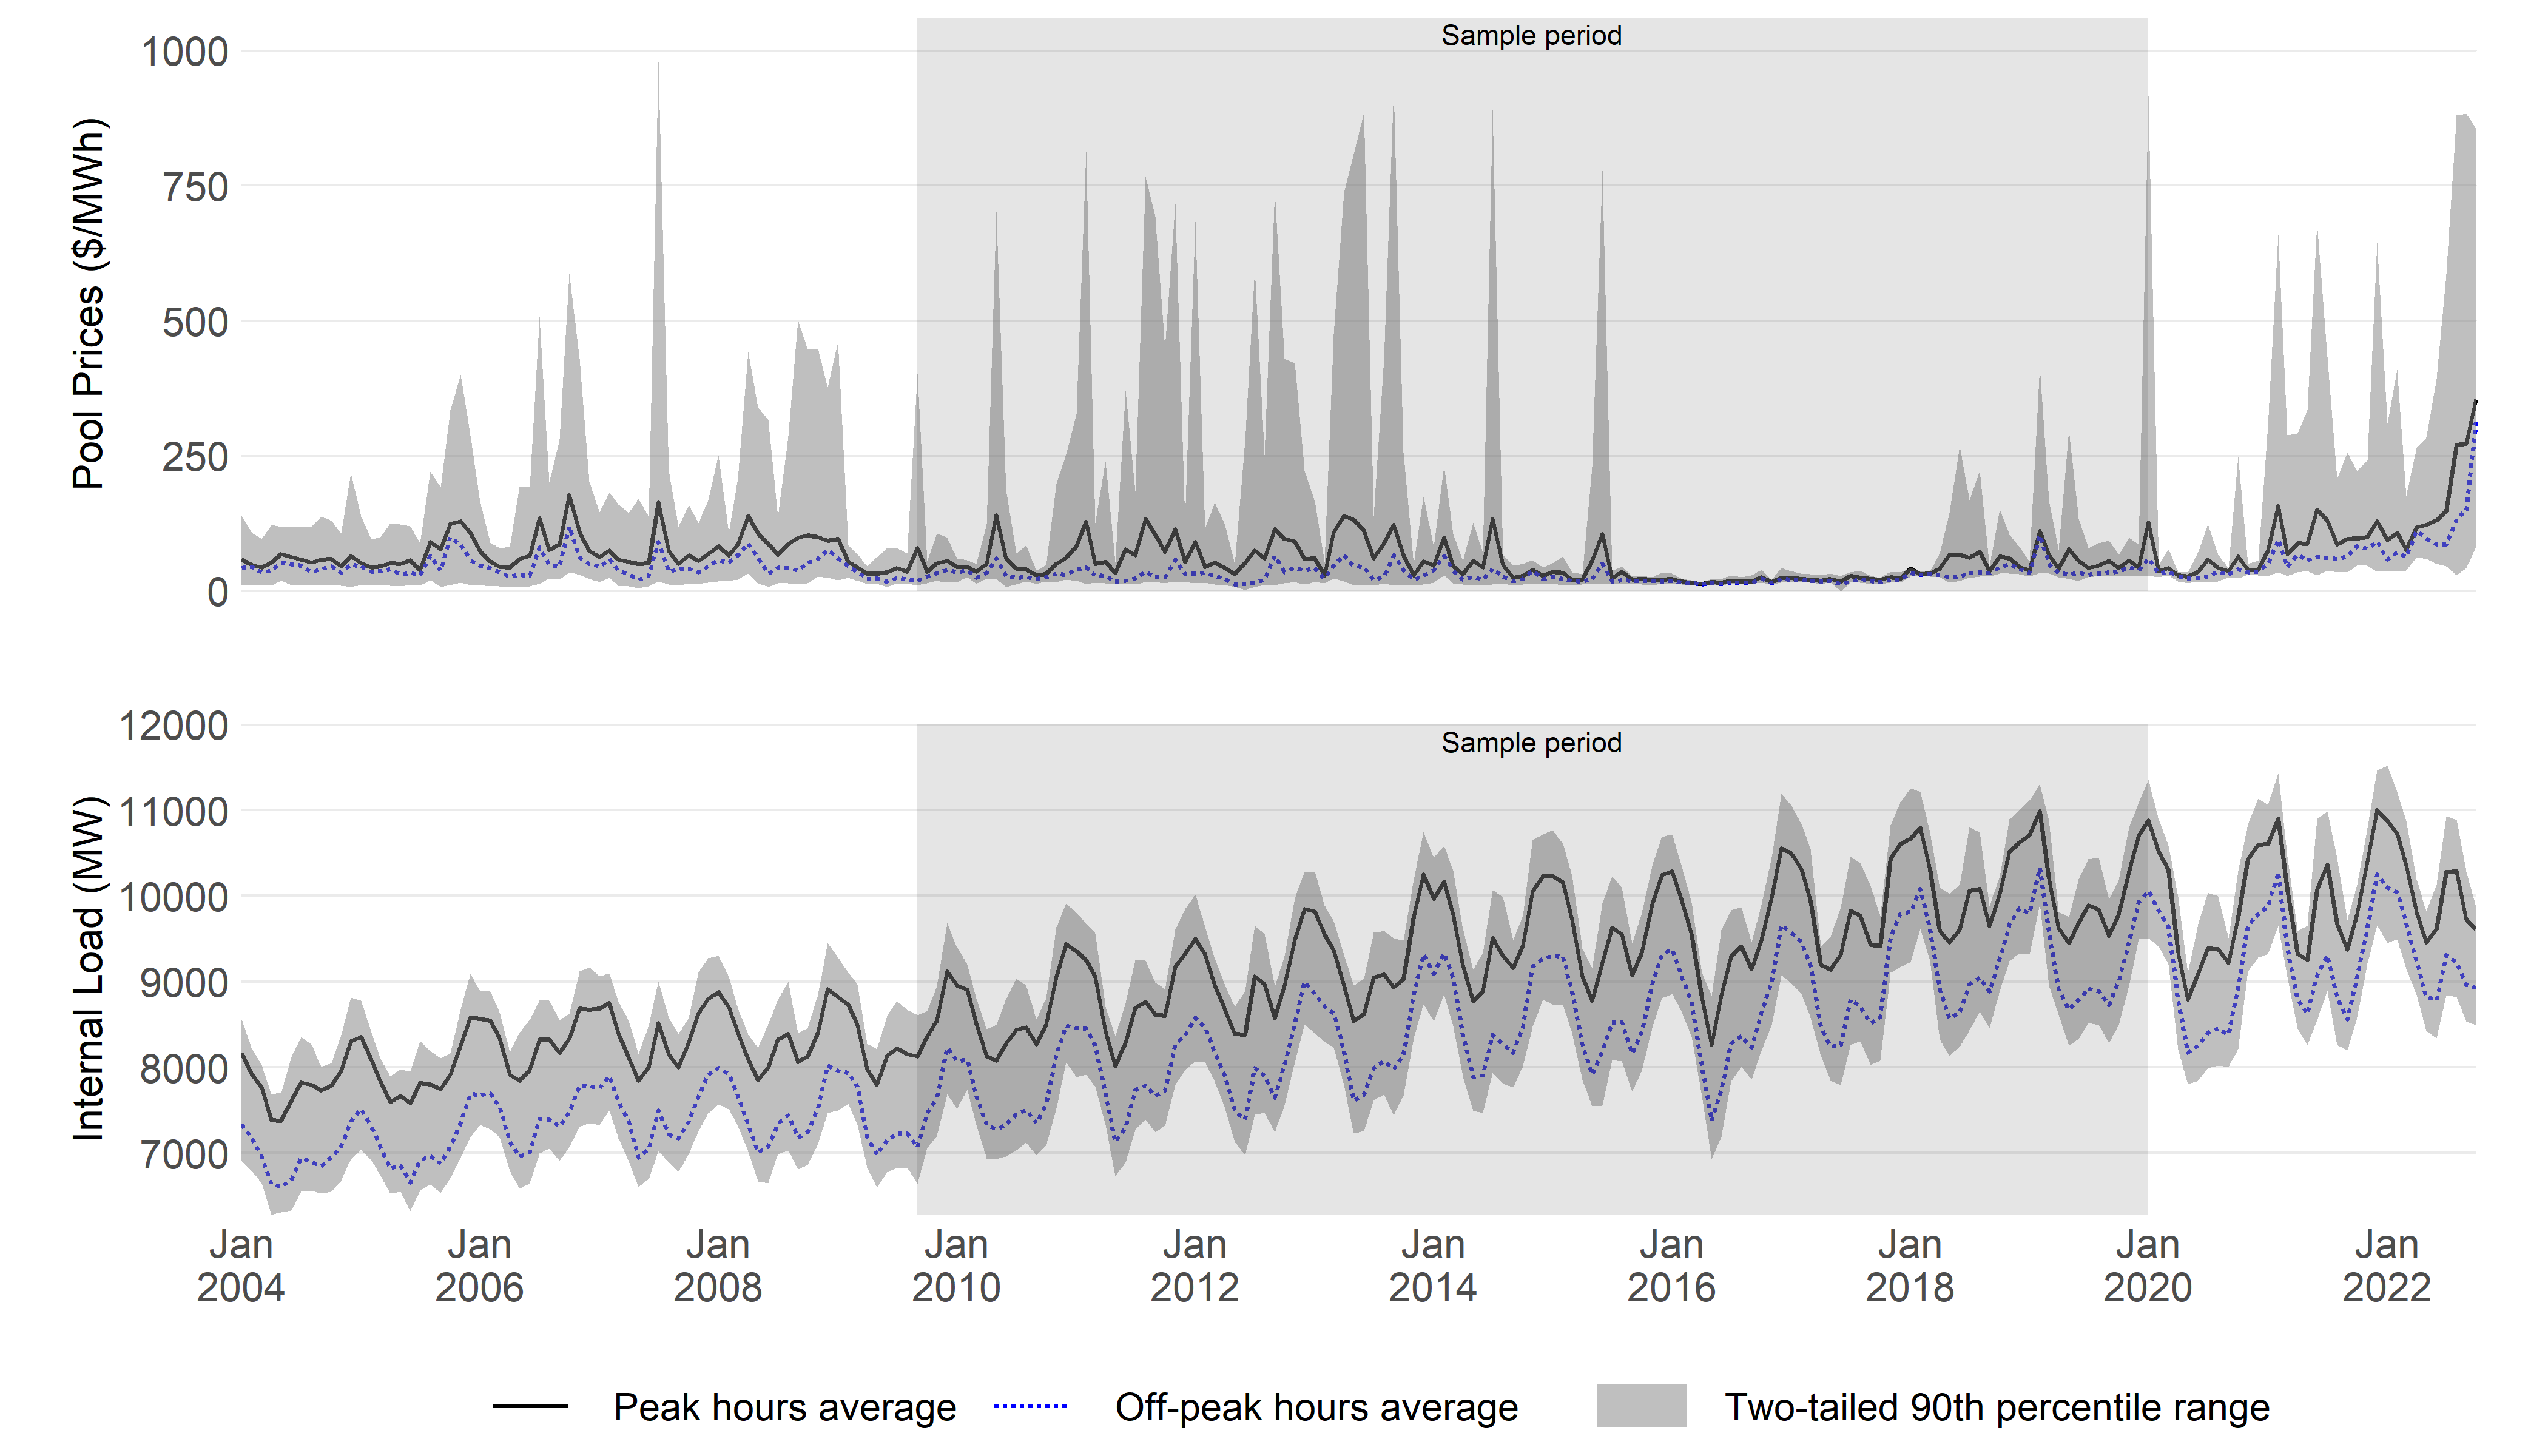
\includegraphics[width=.9\paperwidth]{../images/prices_and_loads.png}}; \vspace{1cm}
   \vfill
\end{frame}


\begin{frame}{Price Volatility}
   \tikz [remember picture,overlay]
    \node[yshift=-.5cm,xshift=0cm] at (current page.center)
        {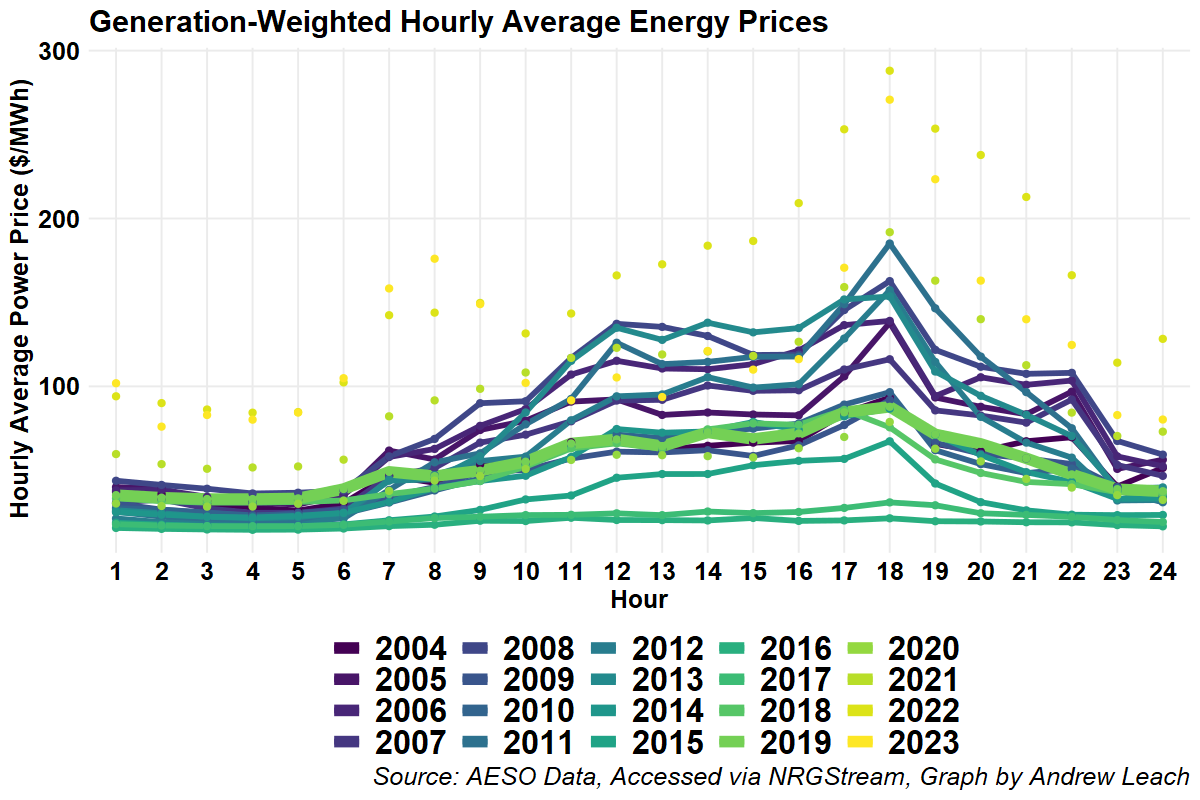
\includegraphics[width=.9\paperwidth]{../images/hourly-prices.png}}; \vspace{1cm}
   \vfill
\end{frame}


\begin{frame}{Growth}
   \tikz [remember picture,overlay]
    \node[yshift=-.5cm,xshift=0cm] at (current page.center)
        {\includegraphics[width=.9\paperwidth]{../images/load_time.png}}; \vspace{1cm}
   \vfill
\end{frame}


\begin{frame}{New Technology}
   \tikz [remember picture,overlay]
    \node[yshift=-.5cm,xshift=0cm] at (current page.center)
        {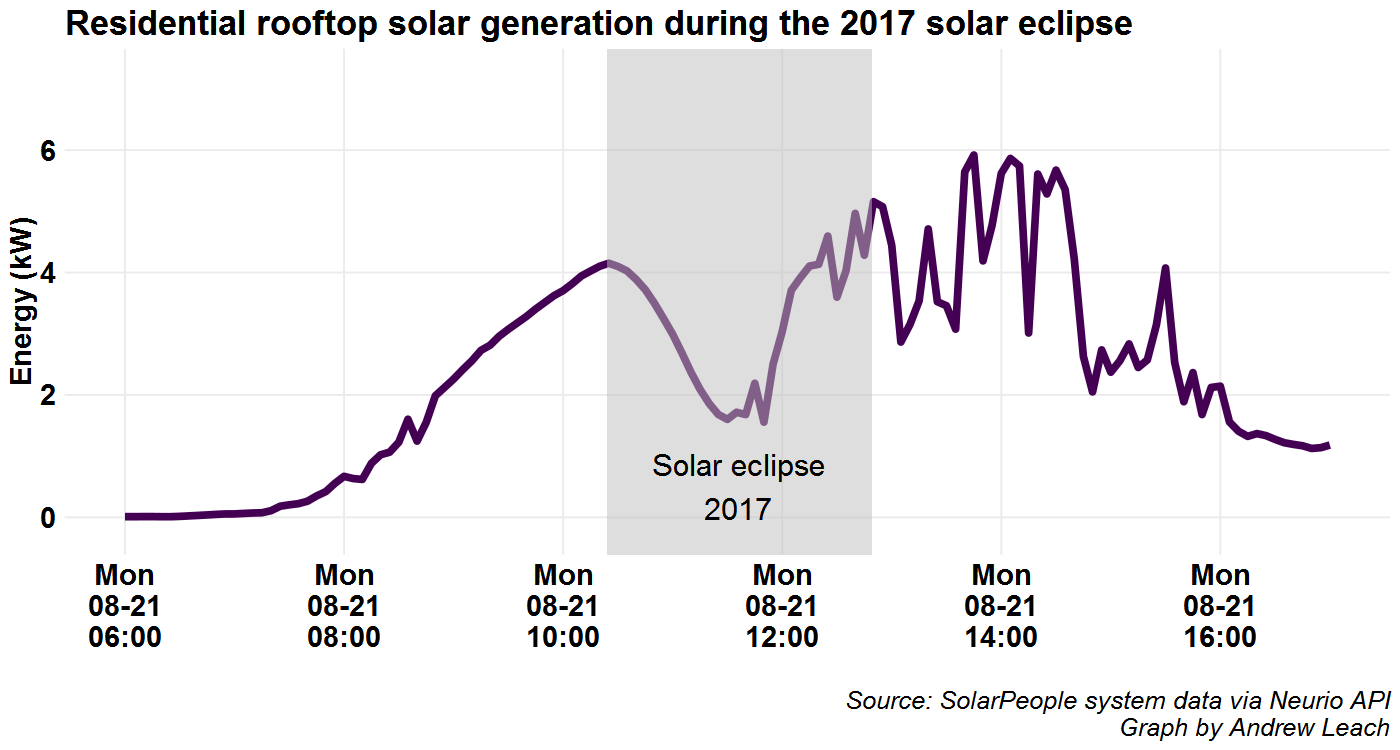
\includegraphics[width=.9\paperwidth]{../images/eclipse.png}}; \vspace{1cm}
   \vfill
\end{frame}


\begin{frame}{Economics 101}
   \tikz [remember picture,overlay]
    \node[yshift=-.5cm,xshift=0cm] at (current page.center)
        {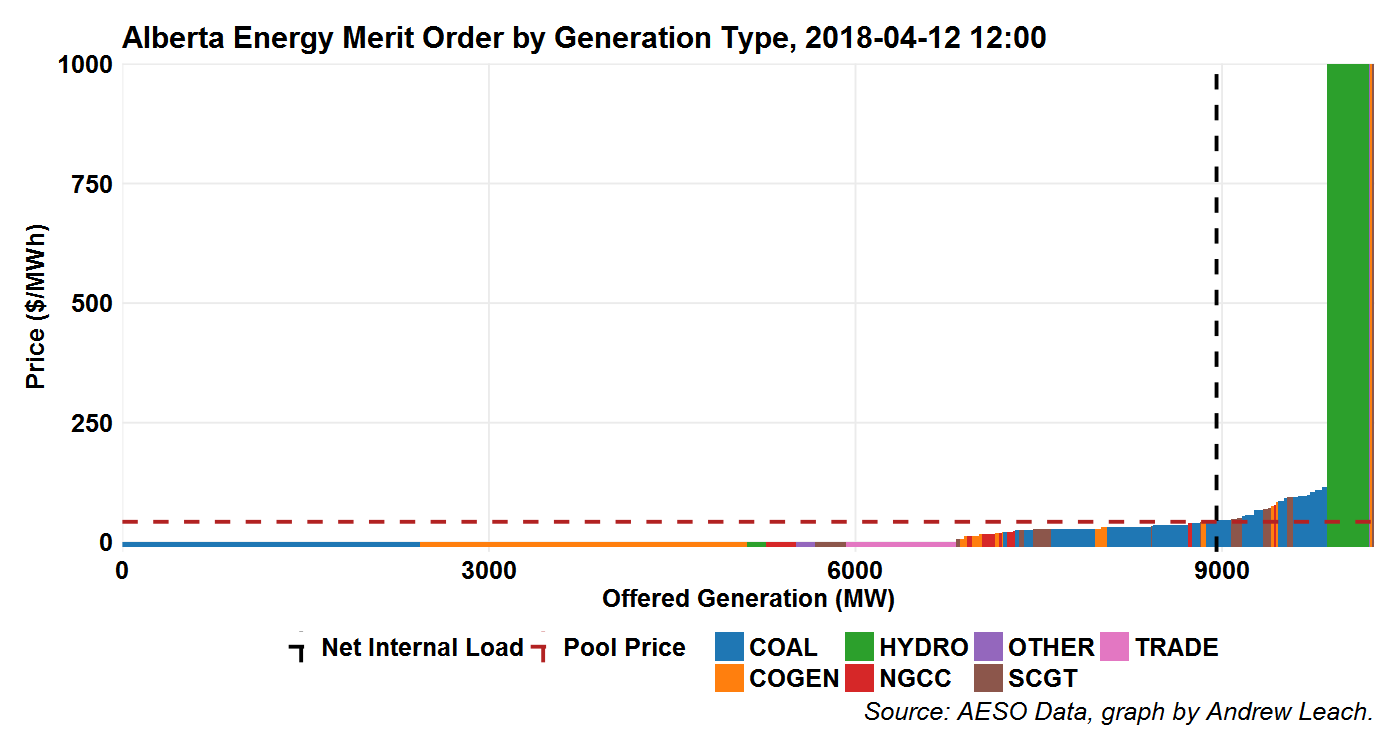
\includegraphics[width=.9\paperwidth]{../images/merit_type.png}}; \vspace{1cm}
   \vfill
\end{frame}

\begin{frame}{Economics 101}
   \tikz [remember picture,overlay]
    \node[yshift=-.5cm,xshift=0cm] at (current page.center)
        {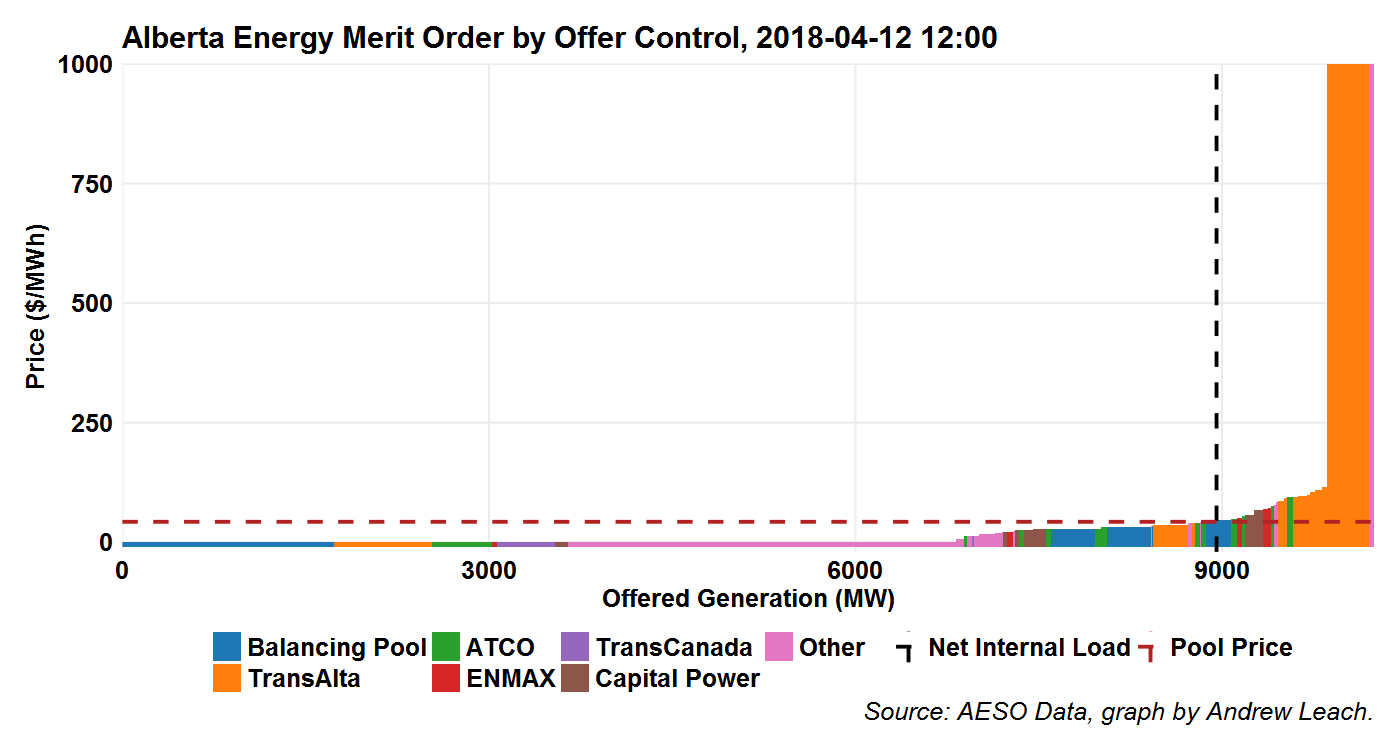
\includegraphics[width=.9\paperwidth]{../images/merit_offer.png}}; \vspace{1cm}
   \vfill
\end{frame}


\begin{frame}

\begin{tabular}{p{\linewidth}}
    \centering
    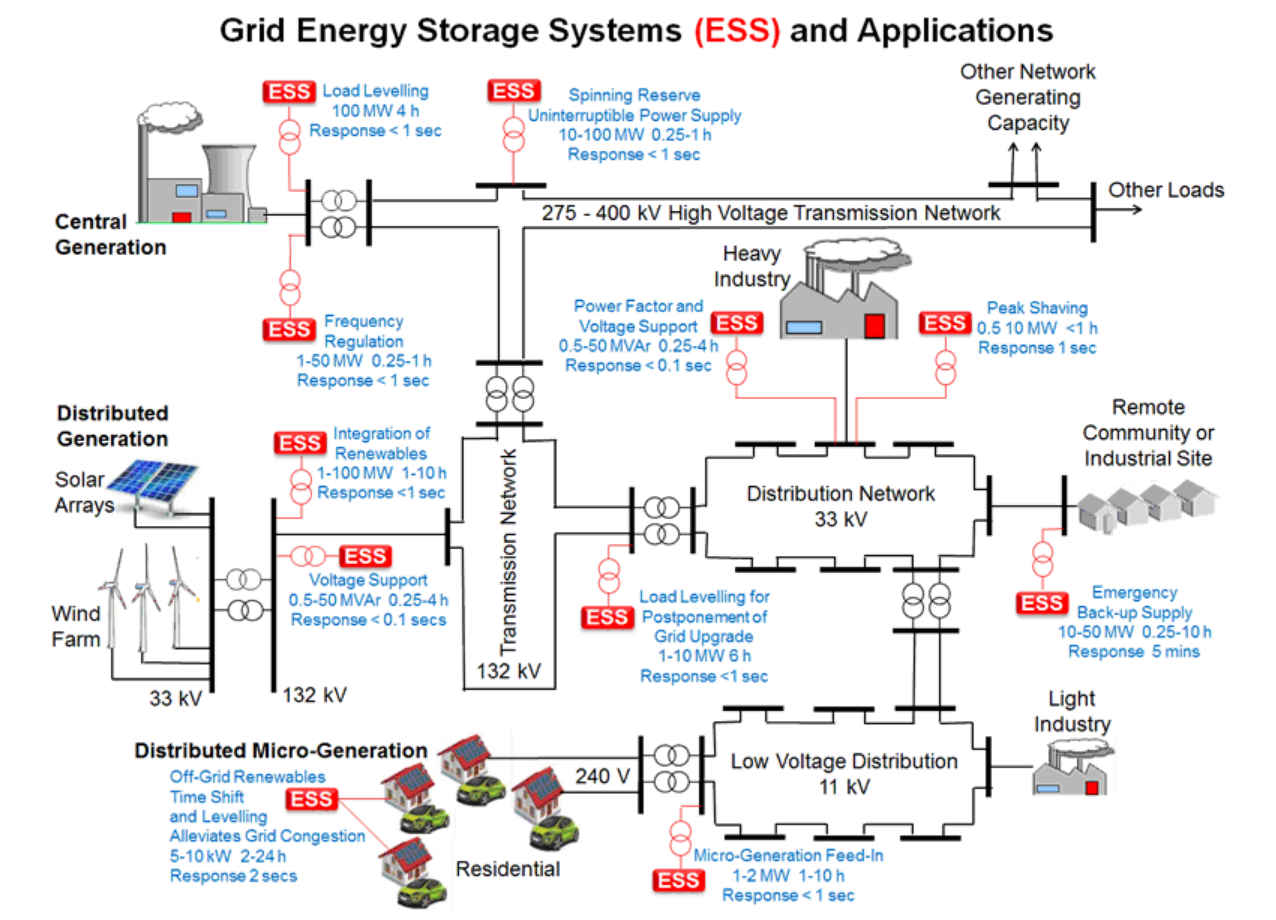
\includegraphics[width=.9\linewidth]{../images/grid_ess.png} \\[\abovecaptionskip]
  Source: \url{http://www.mpoweruk.com/grid_storage.htm}
\end{tabular}

\end{frame}

\begin{frame}{Market Participants}
\begin{itemize}
\setlength\itemsep{1.7em}
\item Generation

\item Transmission

\item Distribution

\item Ancillary Services

\item Load

\item Storage

\item Microgeneration
\end{itemize}

\vfill \end{frame}



\section{Units}

\begin{frame}{Energy units - electricity}
\begin{itemize}
\setlength\itemsep{.75em}
\item Watts: measure of capacity (instantaneous production, installed capacity, or instantaneous demand)
\begin{itemize}
\setlength\itemsep{.5em}
\item Alberta system demand: 7,200-10,700 MW (million watts)
\item Capital Power's Genessee 3 power plant has a nameplate capacity of 450 MW
\end{itemize}
\item Watt hours: measure of energy (production or demand during a given period of time; i.e. flow through)
\begin{itemize}
\setlength\itemsep{.5em}
\item Production over a day, week, month, year
\end{itemize}
\item Volts: measure of the electrical potential or the ability to convert charge to power (Watts=amps x volts)
\begin{itemize}
\setlength\itemsep{.5em}
\item Transmission lines: 150-765 kV
\item Distribution lines: 13,800 Volts
\item Household wiring: 120-240 Volts
\end{itemize}
\end{itemize}
\vfill \end{frame}

\begin{frame}{Energy Prices}
\begin{itemize}
\setlength\itemsep{.25em}
\item Electricity prices: expressed in power delivered over time
\begin{itemize}
\setlength\itemsep{.15em}
\item Cents/kilowatt-hour (c/kWh)
\item Dollars per megawatt-hour (\$/MWh)
\item Levelized costs of electricity (supply costs) in \$/MWh
\end{itemize}

\item Capacity costs are expressed in a cost per megawatt or cost of capacity
\begin{itemize}
\setlength\itemsep{.15em}
\item Genessee 3 cost approximately \$1.5 million/MW or \$1.50 per watt to build
\item Solar panel prices have declined to now lie under \$1/W of capacity
\item Balance of system costs imply that a solar system costs \$2-3/W of installed capacity
\end{itemize}
\item Other prices matter for electricity markets as well
\begin{itemize}
\setlength\itemsep{.15em}
\item Renewable energy credits (usually prices in \$/MWh)
\item Emissions credits or permits (\$/tonne)
\item Capacity payments (\$/MW)
\item Air emissions permits or credits (\$/tonne)
\end{itemize}
\end{itemize}

\vfill \end{frame}

\section{Power Markets}

\begin{frame}{Regulatory characteristics}
\begin{itemize}
\setlength\itemsep{.25em}
\item Rate-regulated or or state-owned utilities
\item Competitive markets
\begin{itemize}
\setlength\itemsep{.15em}
\item Energy only markets: ERCOT and Alberta
\item Energy and capacity markets: MISO, PJM, soon-to-be Alberta
\item Real-time vs day-ahead prices: PJM and others have day-ahead market and then a real time differences market
\item Many other design characteristic differences between restructured or competitive markets
\end{itemize}
\end{itemize}

\vfill
\end{frame}


\begin{frame}{Alberta Market Design}
\begin{itemize}
\setlength\itemsep{.25em}
\item Energy-only market
\item Real time, spot pricing, no day-ahead market
\item Single node
\item Capacity market to be added in the near future
\item Transmission
\item Congestion free (no nodal pricing)
\item No transmission rights
\item Ancillary services: separate, competitive market for operating reserves, transmission-must-run, load-shed and black start
\end{itemize}

\vfill
\end{frame}


\begin{frame}{Nodal Pricing Example}

\begin{tabular}{p{\linewidth}}
    \centering
    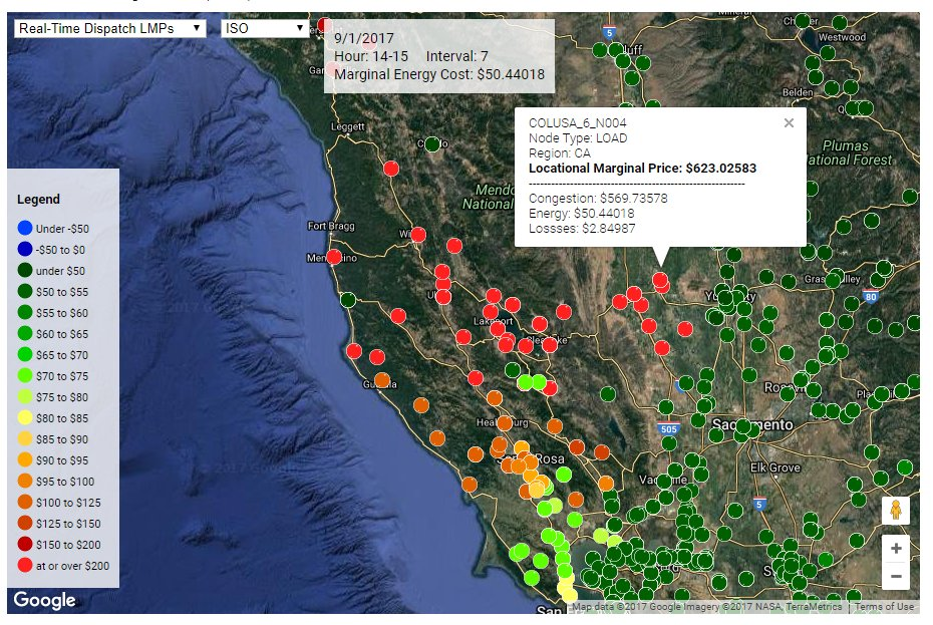
\includegraphics[width=\linewidth]{../images/cali_nodes.png} \\[.1\abovecaptionskip]
  Source: CAISO
\end{tabular}
\vfill
\end{frame}

\section{Wholesale Market}

\begin{frame}{The Wholesale Market}
\begin{itemize}
\setlength\itemsep{2em}
\item Suppliers place offers of power at particular price
\item Demand-side bids placed for power with a maximum price
\item Supply offers are sorted from low to high
\item Demand offers are sorted from high to low
\item Marginal price is set at the price which equates supply and demand - economics 101 at work!
\item Import supply is bid-in at \$0, but receive the marginal price
\item Export demand is bid-in at \$999, so they do not set the price directly but pay the marginal price
\item Consumer default bid allows AESO to go up merit order to meet observed demand
\end{itemize}

\vfill \end{frame}

\begin{frame}{The Merit Order}
   \tikz [remember picture,overlay]
    \node[yshift=-.5cm,xshift=0cm] at (current page.center)
        {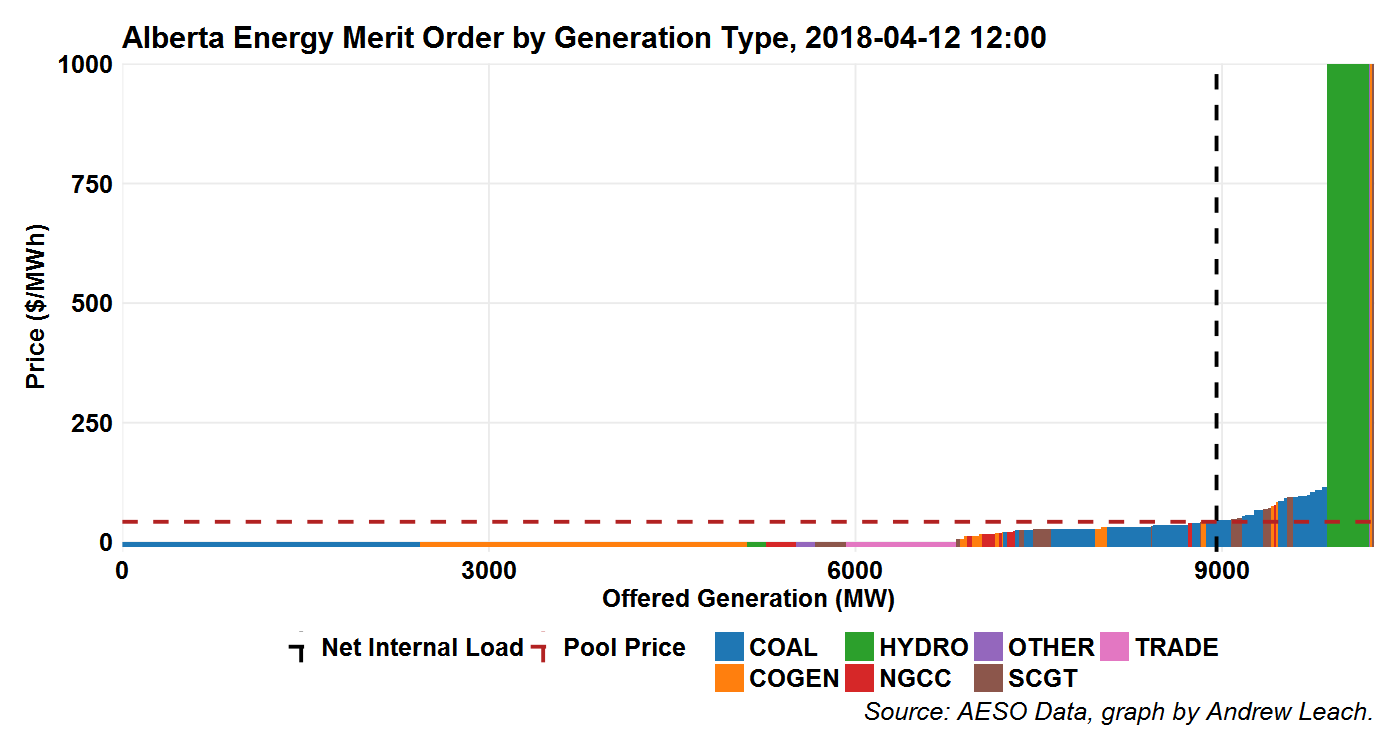
\includegraphics[width=.9\paperwidth]{../images/merit_type.png}}; \vspace{1cm}
   \vfill
\end{frame}

\begin{frame}{The Merit Order}
   \tikz [remember picture,overlay]
    \node[yshift=-.5cm,xshift=0cm] at (current page.center)
        {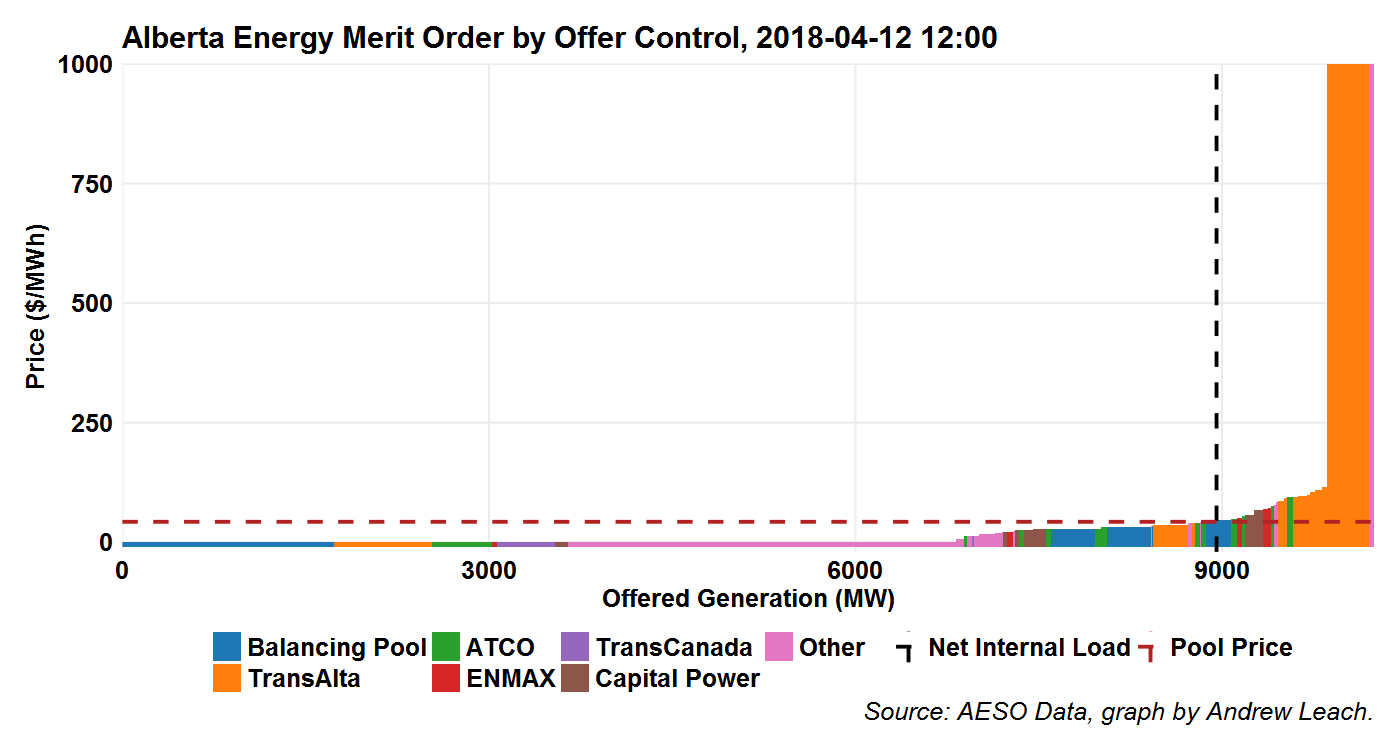
\includegraphics[width=.9\paperwidth]{../images/merit_offer.png}}; \vspace{1cm}
   \vfill
\end{frame}

\begin{frame}{Offers}
   \tikz [remember picture,overlay]
    \node[yshift=-.5cm,xshift=0cm] at (current page.center)
        {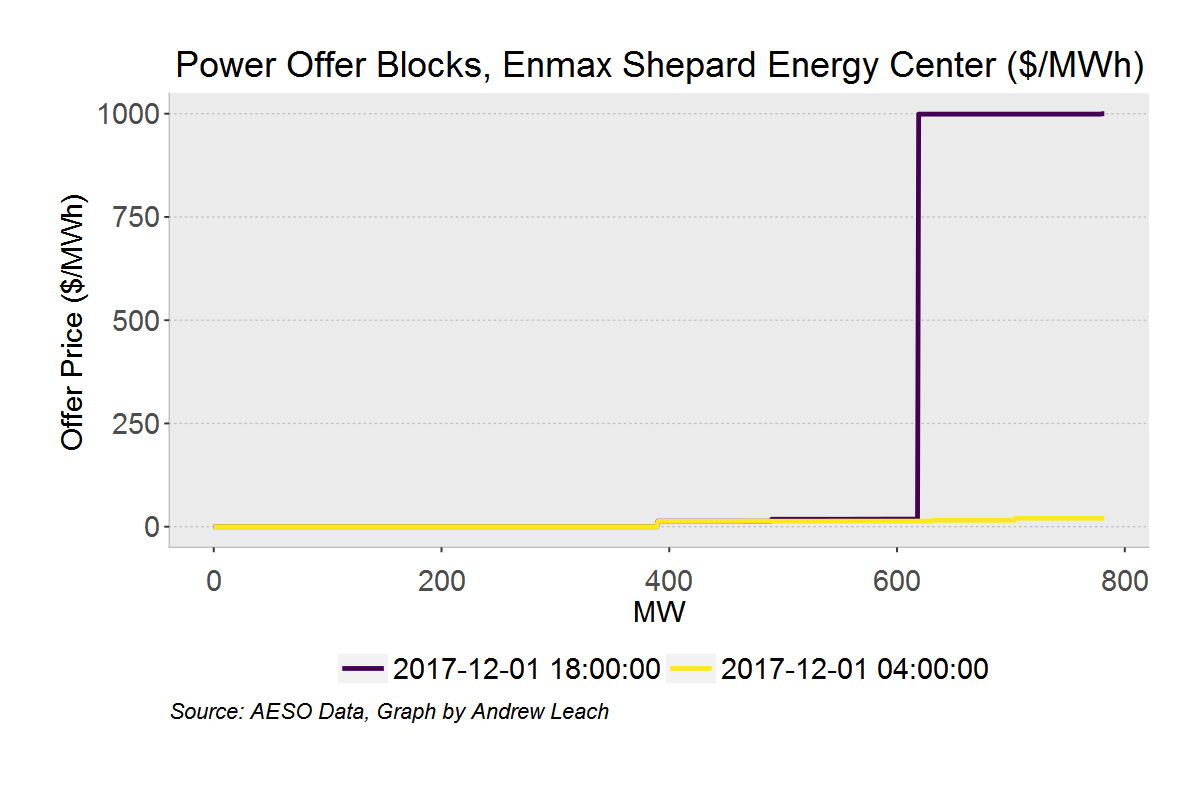
\includegraphics[width=.9\paperwidth]{../images/bids.png}}; \vspace{1cm}
   \vfill
\end{frame}

\begin{frame}{Offers}
   \tikz [remember picture,overlay]
    \node[yshift=-.5cm,xshift=0cm] at (current page.center)
        {
\includegraphics[width=.9\paperwidth]{../images/bids_alpac.png}}; \vspace{1cm}
   \vfill
\end{frame}


\begin{frame}{Hourly Loads}
   \tikz [remember picture,overlay]
    \node[yshift=-.5cm,xshift=0cm] at (current page.center)
        {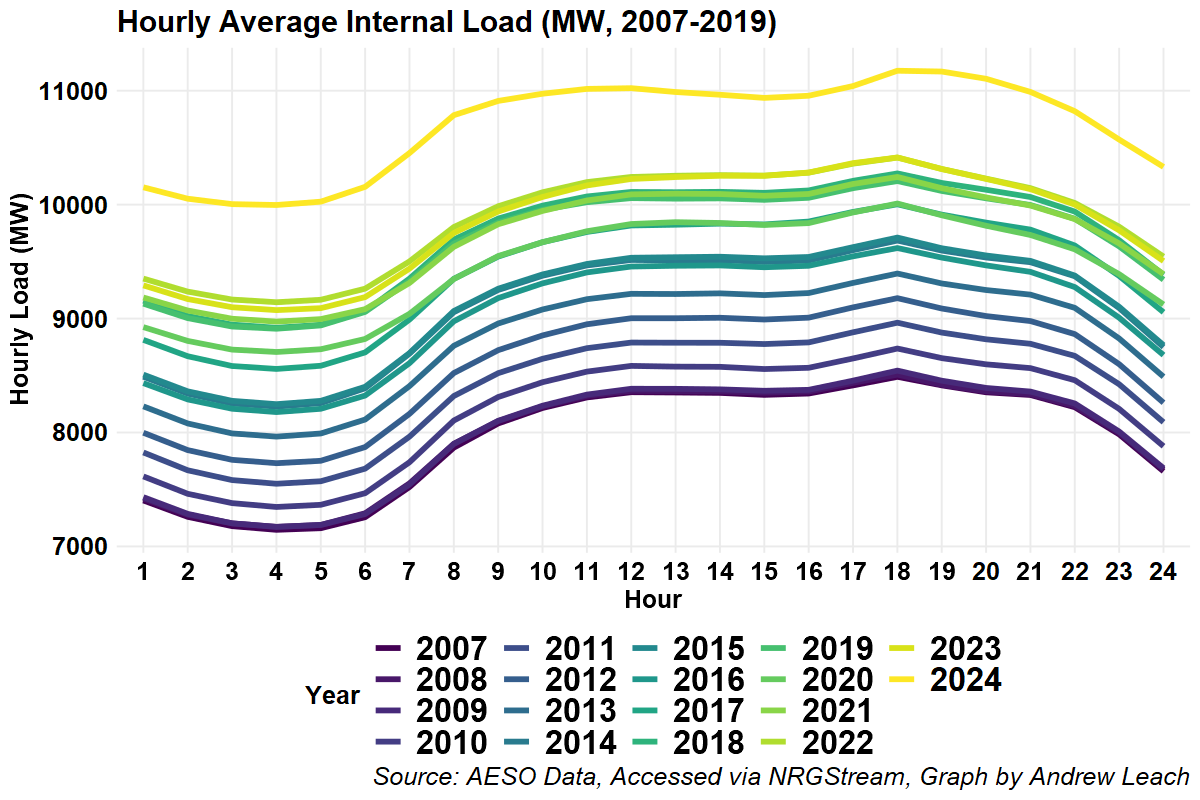
\includegraphics[width=.9\paperwidth]{../images/hourly-loads.png}}; \vspace{1cm}
   \vfill
\end{frame}


\begin{frame}{Monthly Peak Loads}
   \tikz [remember picture,overlay]
    \node[yshift=-.5cm,xshift=0cm] at (current page.center)
        {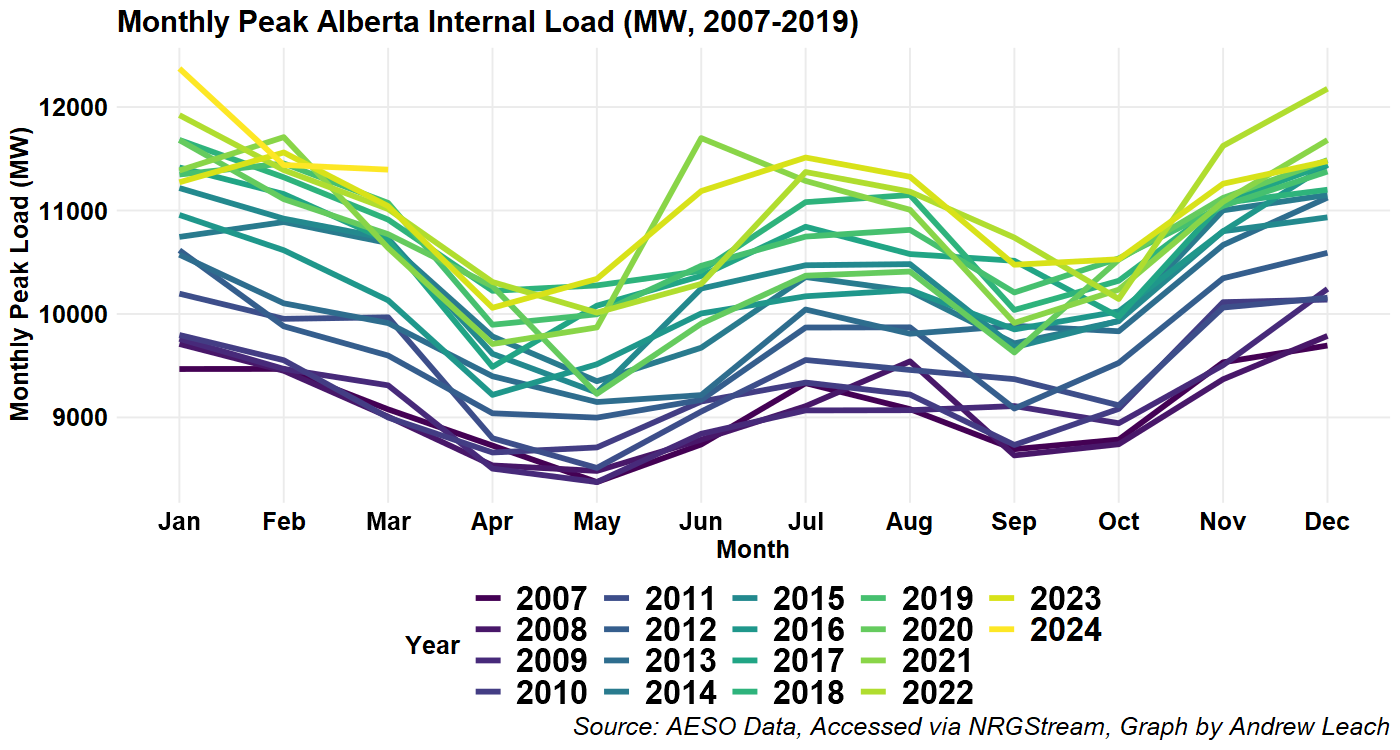
\includegraphics[width=.9\paperwidth]{../images/monthly-peak-loads.png}}; \vspace{1cm}
   \vfill
\end{frame}


\begin{frame}{Monthly Average Loads}
   \tikz [remember picture,overlay]
    \node[yshift=-.5cm,xshift=0cm] at (current page.center)
        {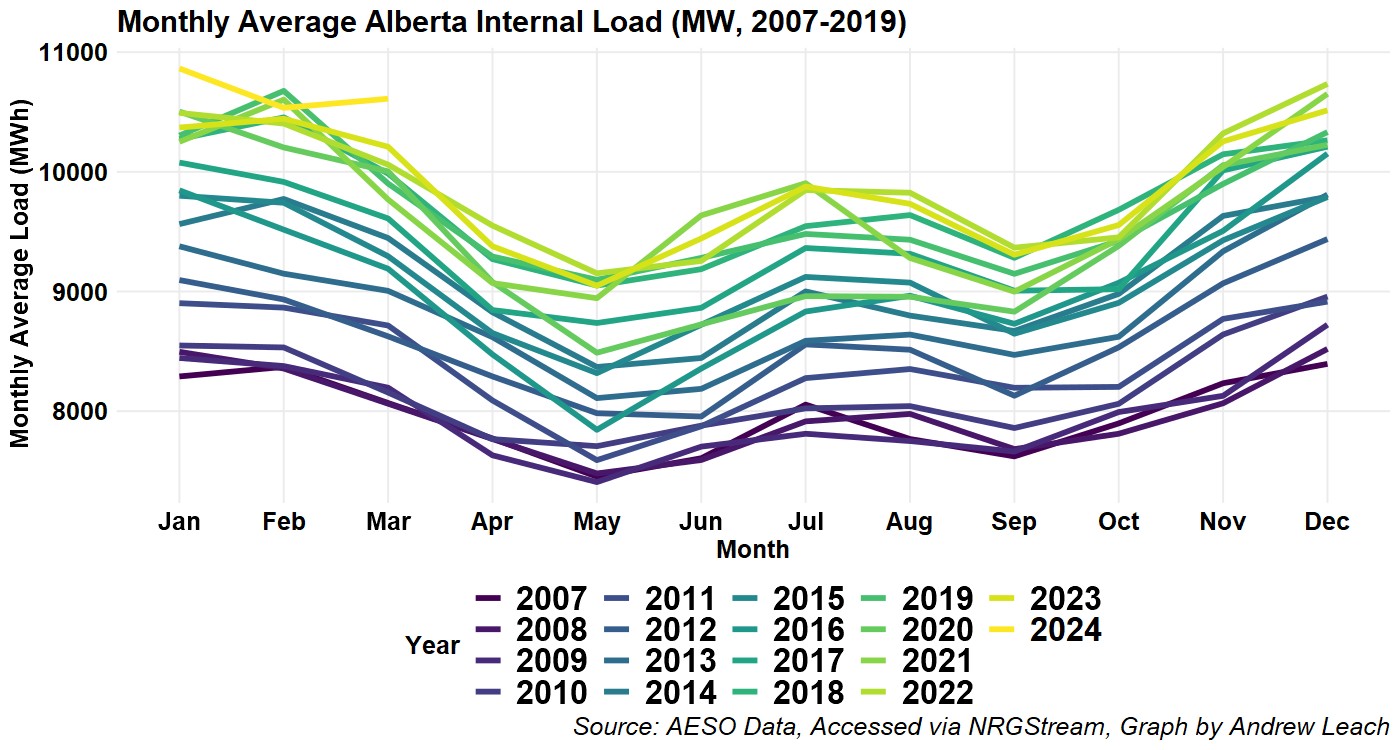
\includegraphics[width=.9\paperwidth]{../images/monthly-avg-loads.png}}; \vspace{1cm}
   \vfill
\end{frame}



\begin{frame}{Hourly Prices}
   \tikz [remember picture,overlay]
    \node[yshift=-.5cm,xshift=0cm] at (current page.center)
        {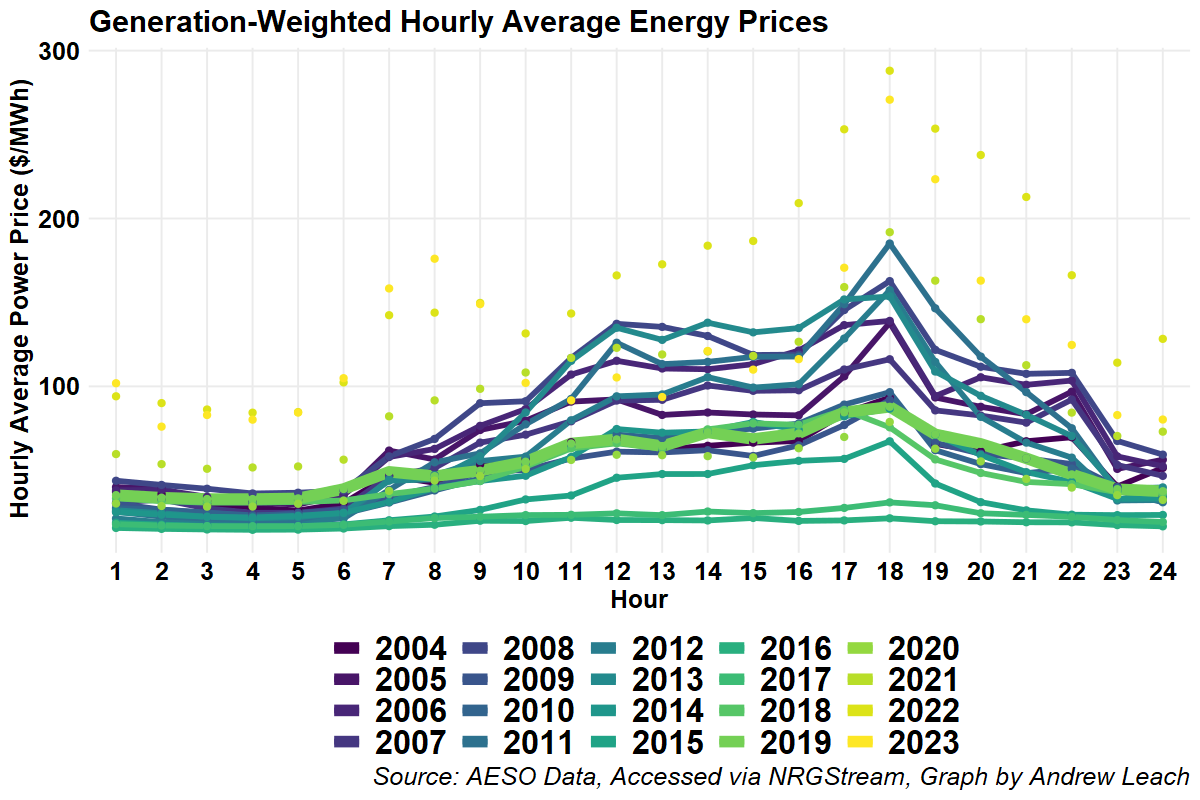
\includegraphics[width=.9\paperwidth]{../images/hourly-prices.png}}; \vspace{1cm}
   \vfill
\end{frame}


\begin{frame}{Recent Hourly Prices}
   \tikz [remember picture,overlay]
    \node[yshift=-.5cm,xshift=0cm] at (current page.center)
        {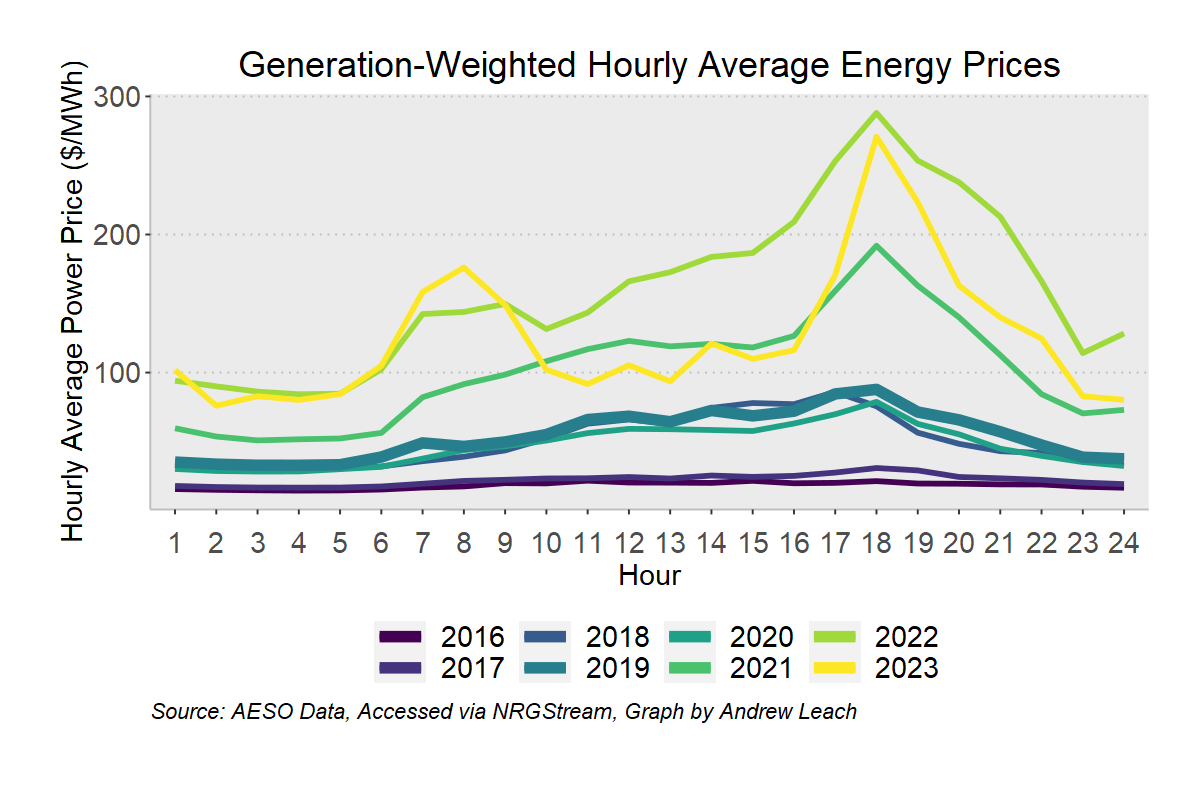
\includegraphics[width=.9\paperwidth]{../images/hourly-prices-recent.png}}; \vspace{1cm}
   \vfill
\end{frame}


\begin{frame}{Prices over time}
   \tikz [remember picture,overlay]
    \node[yshift=-.5cm,xshift=0cm] at (current page.center)
        {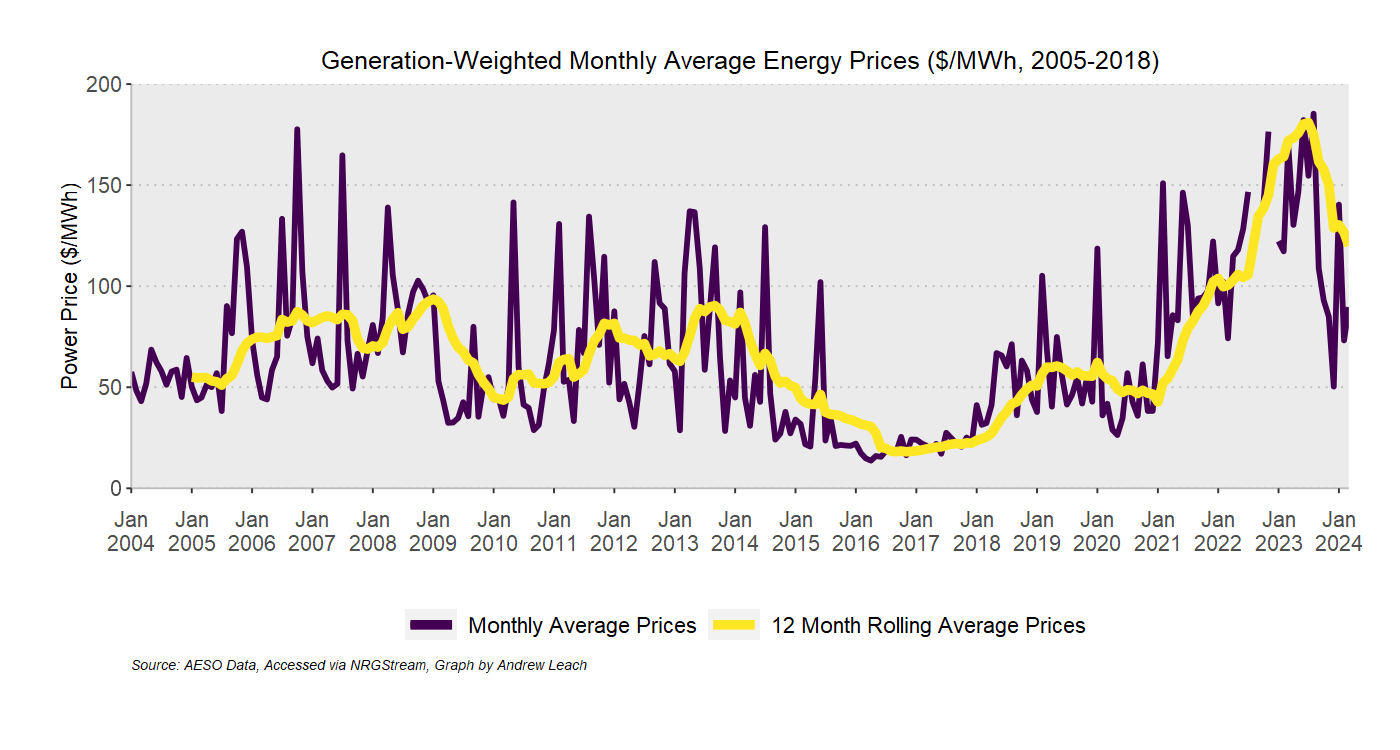
\includegraphics[width=.9\paperwidth]{../images/monthly_prices.png}}; \vspace{1cm}
   \vfill
\end{frame}


\begin{frame}{Prices over time}
   \tikz [remember picture,overlay]
    \node[yshift=-.5cm,xshift=0cm] at (current page.center)
        {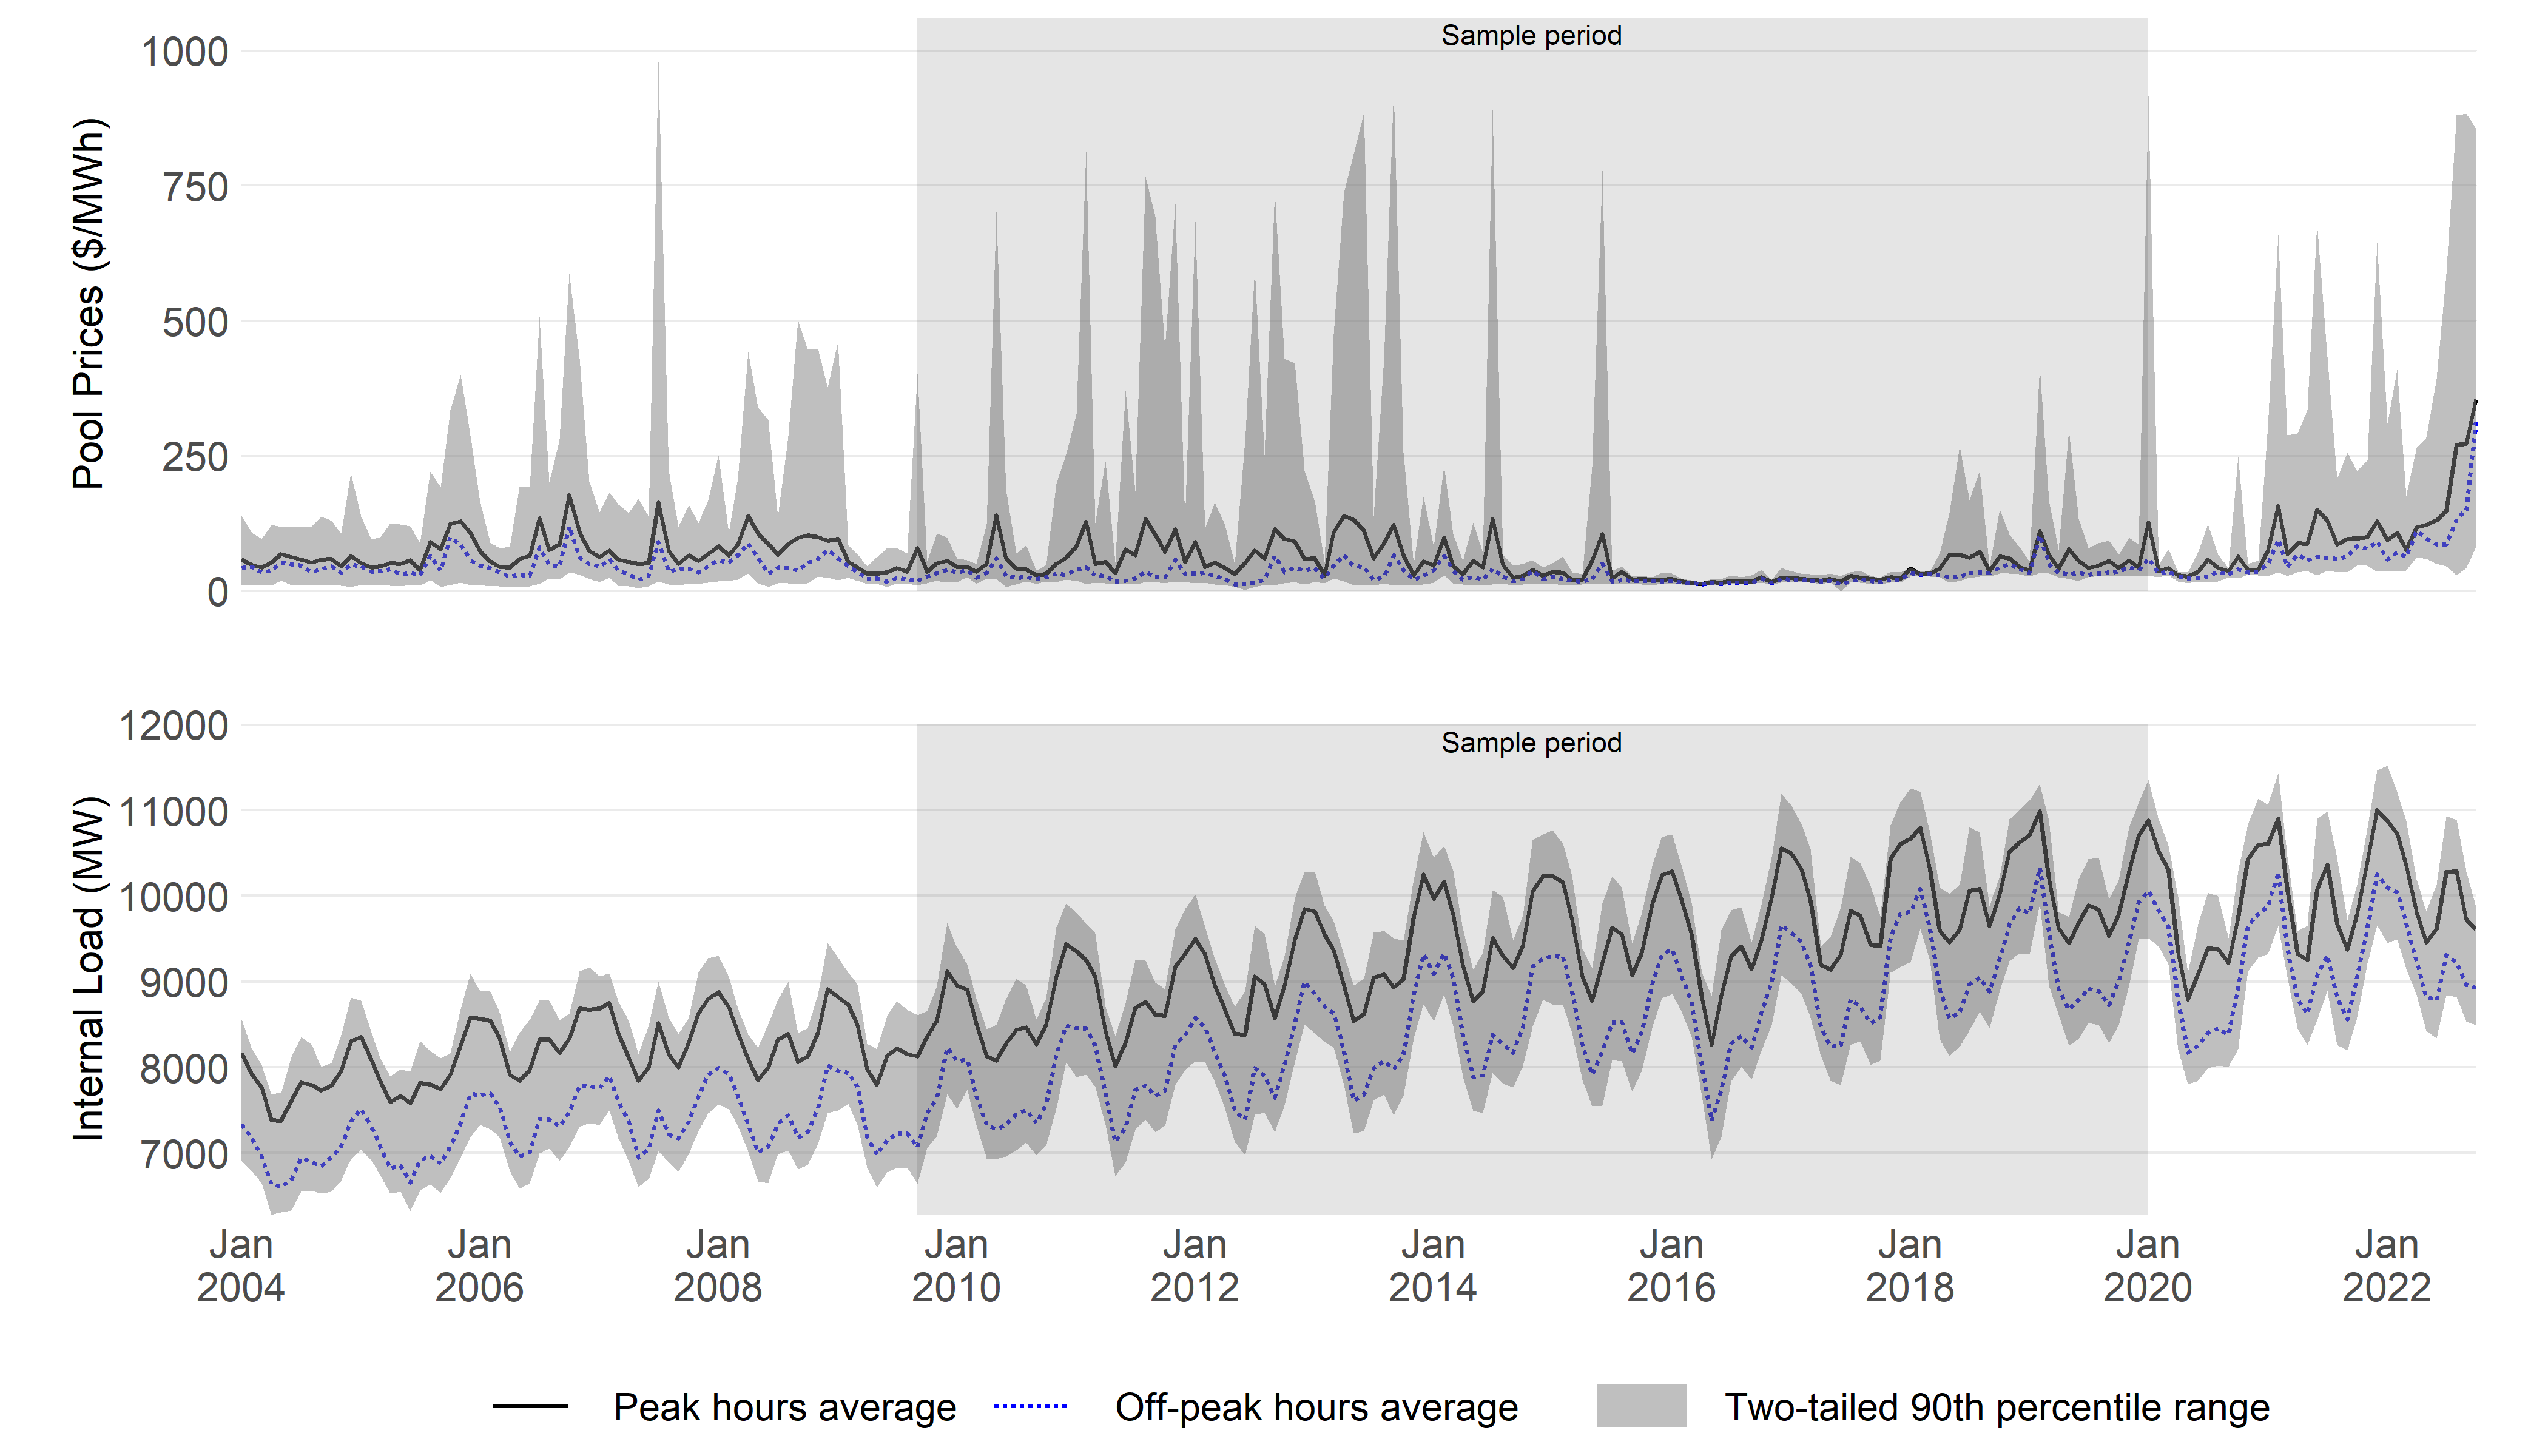
\includegraphics[width=.9\paperwidth]{../images/prices_and_loads.png}}; \vspace{1cm}
   \vfill
\end{frame}


\begin{frame}{Prices over time}
   \tikz [remember picture,overlay]
    \node[yshift=-.5cm,xshift=0cm] at (current page.center)
        {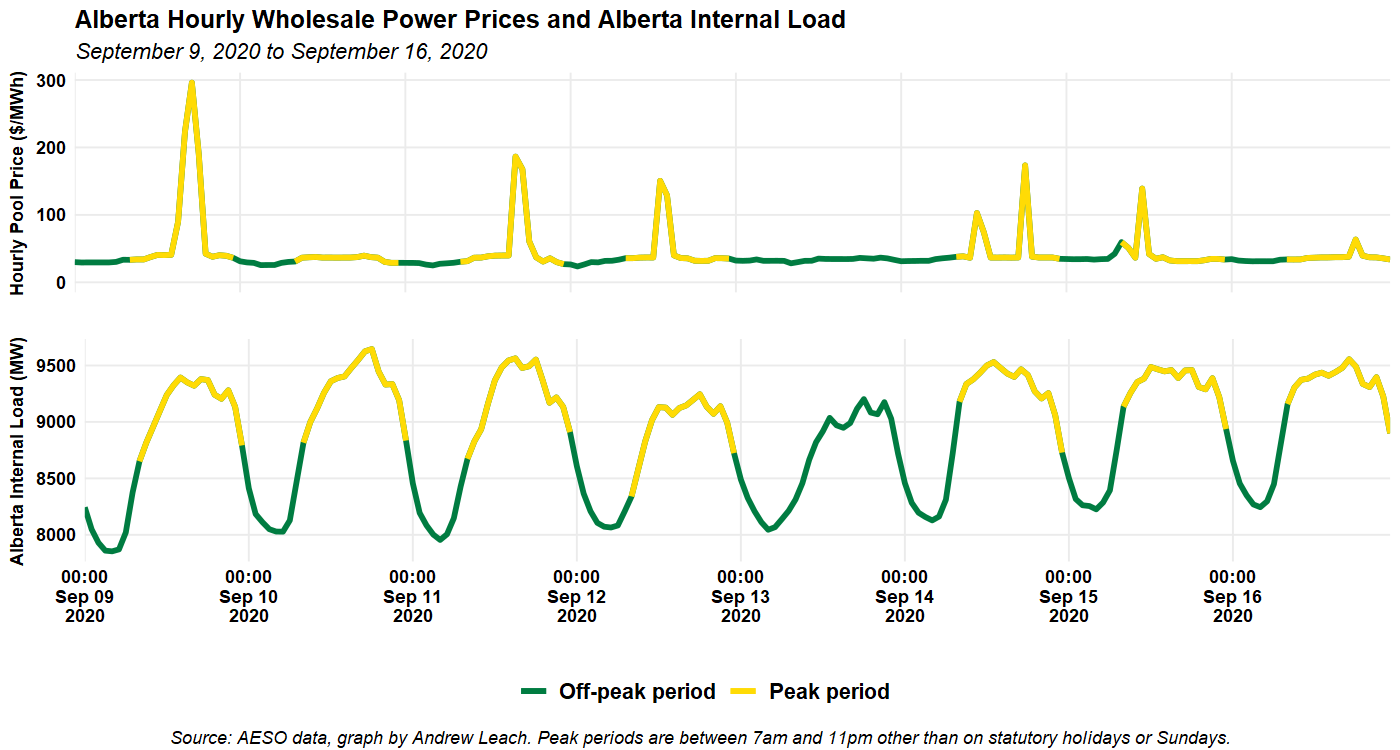
\includegraphics[width=.9\paperwidth]{../images/peak_prices_week.png}}; \vspace{1cm}
   \vfill
\end{frame}


\begin{frame}{Forecasting Prices and Loads}
   \tikz [remember picture,overlay]
    \node[yshift=-.5cm,xshift=0cm] at (current page.center)
        {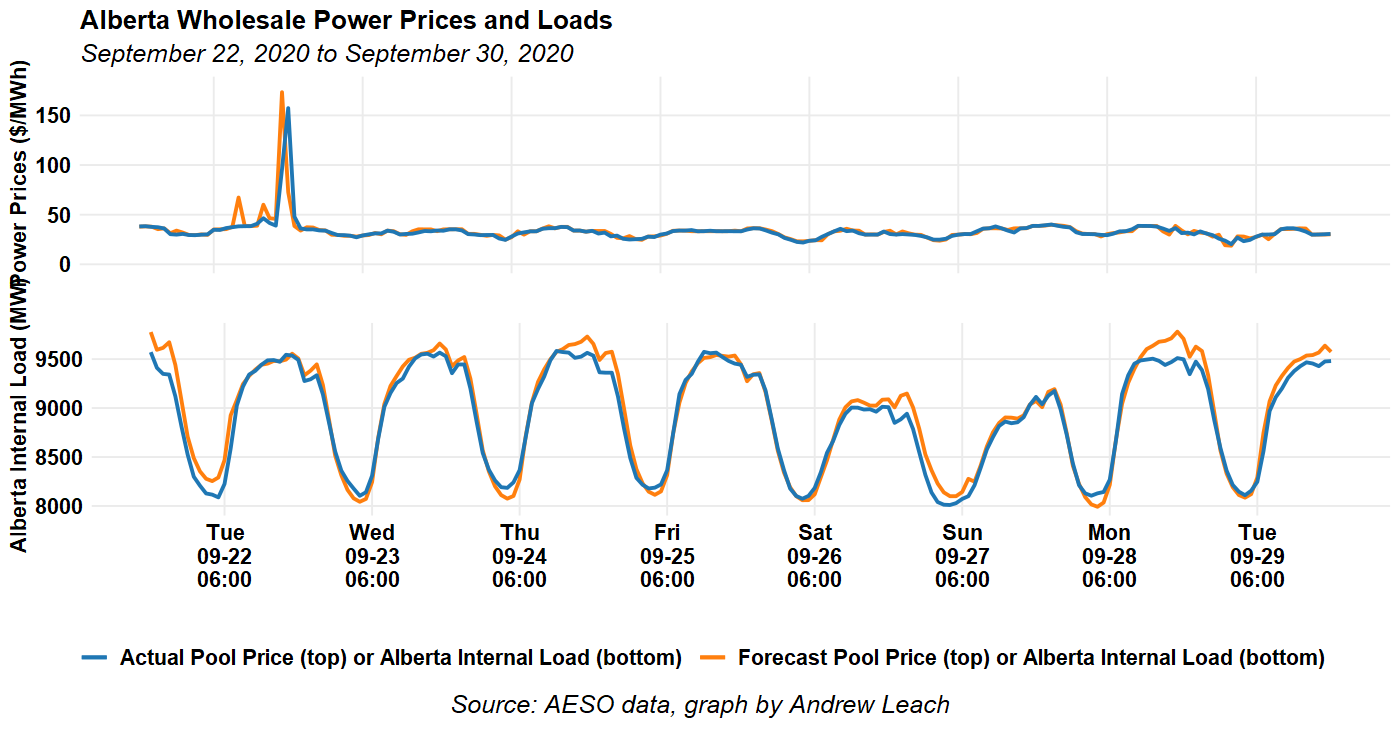
\includegraphics[width=.9\paperwidth]{../images/price_and_load.png}}; \vspace{1cm}
   \vfill
\end{frame}



\begin{frame}{Duration Curve of Prices}
   \tikz [remember picture,overlay]
    \node[yshift=-.5cm,xshift=0cm] at (current page.center)
        {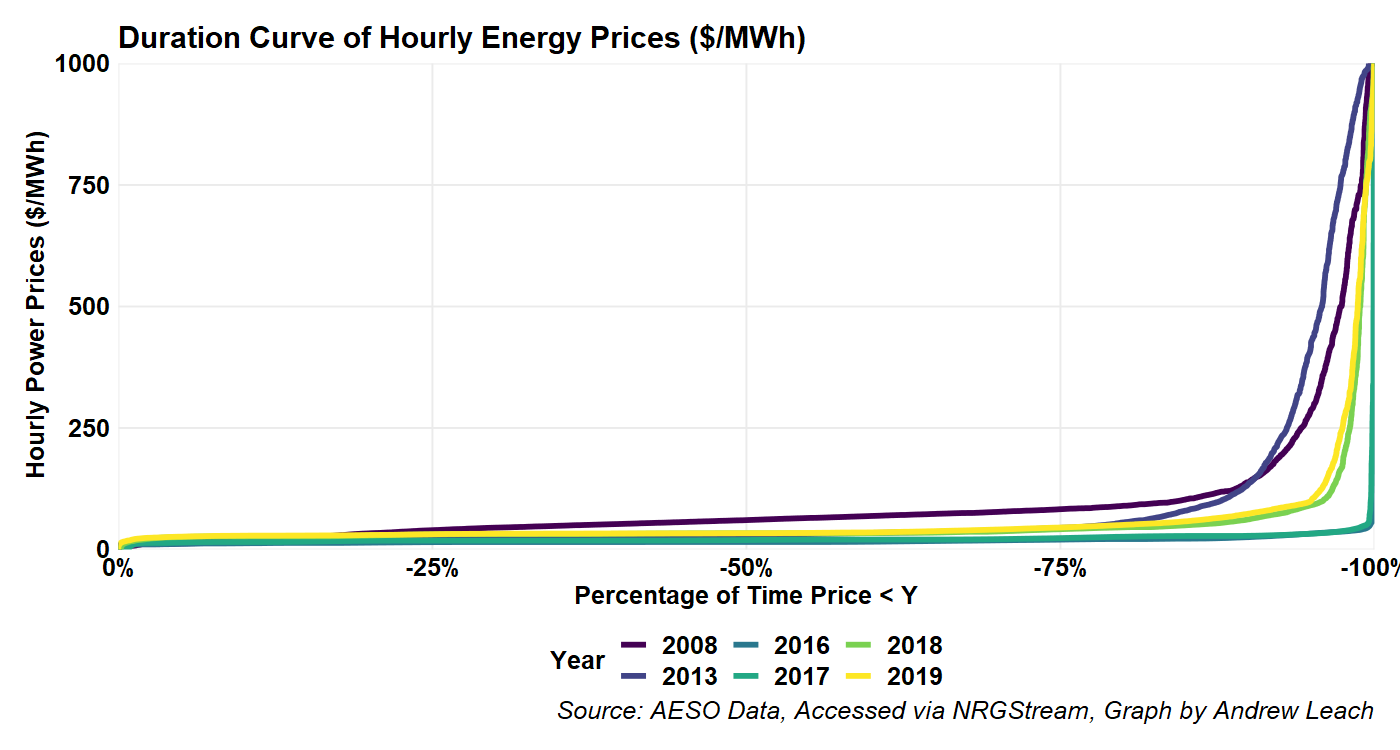
\includegraphics[width=.9\paperwidth]{../images/price_dist.png}}; \vspace{1cm}
   \vfill
\end{frame}

\begin{frame}{Duration Curve of Prices}
   \tikz [remember picture,overlay]
    \node[yshift=-.5cm,xshift=0cm] at (current page.center)
        {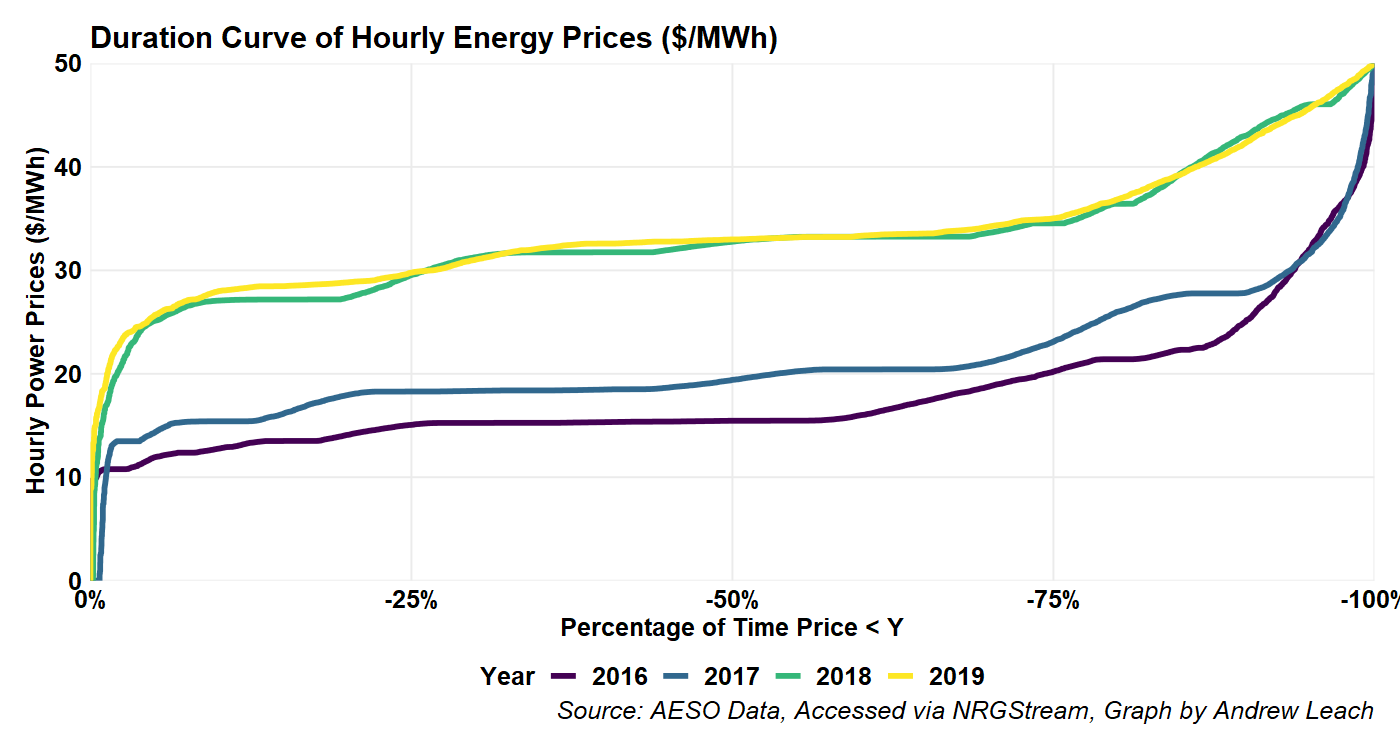
\includegraphics[width=.9\paperwidth]{../images/price_dist_recent.png}}; \vspace{1cm}
   \vfill
\end{frame}



\begin{frame}{Forward Markets}
   \tikz [remember picture,overlay]
    \node[yshift=-.5cm,xshift=0cm] at (current page.center)
        {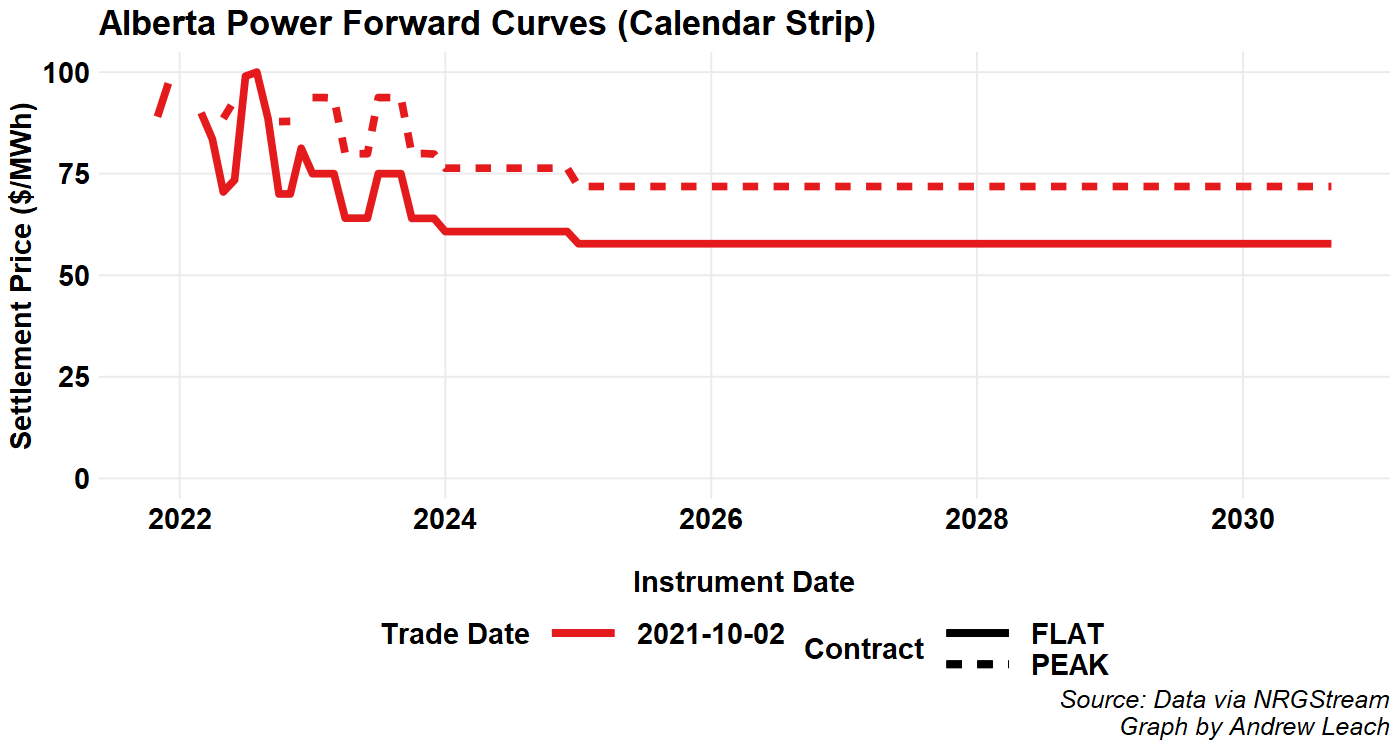
\includegraphics[width=.9\paperwidth]{../images/forwards_all.png}}; \vspace{1cm}
   \vfill
\end{frame}



\begin{frame}{Forward Markets}
   \tikz [remember picture,overlay]
    \node[yshift=-.5cm,xshift=0cm] at (current page.center)
        {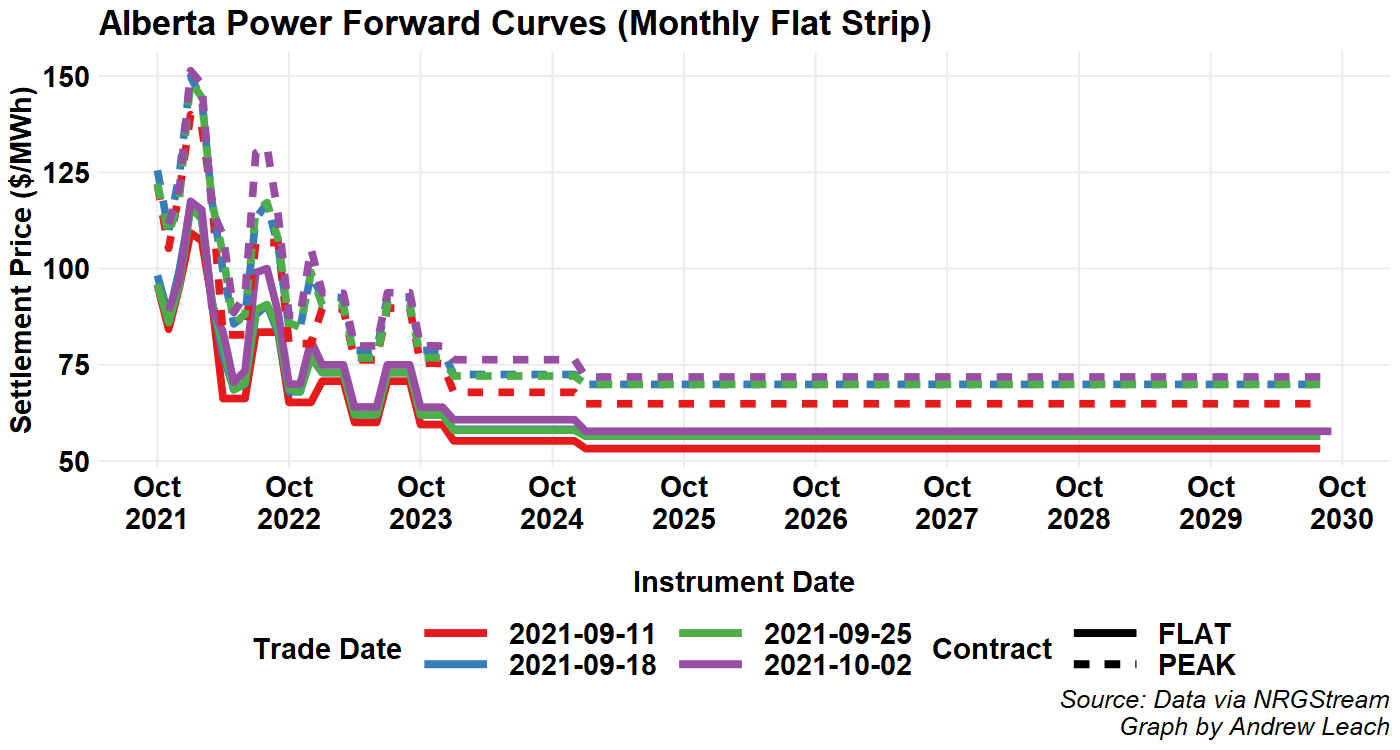
\includegraphics[width=.9\paperwidth]{../images/forwards_monthly.png}}; \vspace{1cm}
   \vfill
\end{frame}

\begin{frame}{Forward Markets}
   \tikz [remember picture,overlay]
    \node[yshift=-.5cm,xshift=0cm] at (current page.center)
        {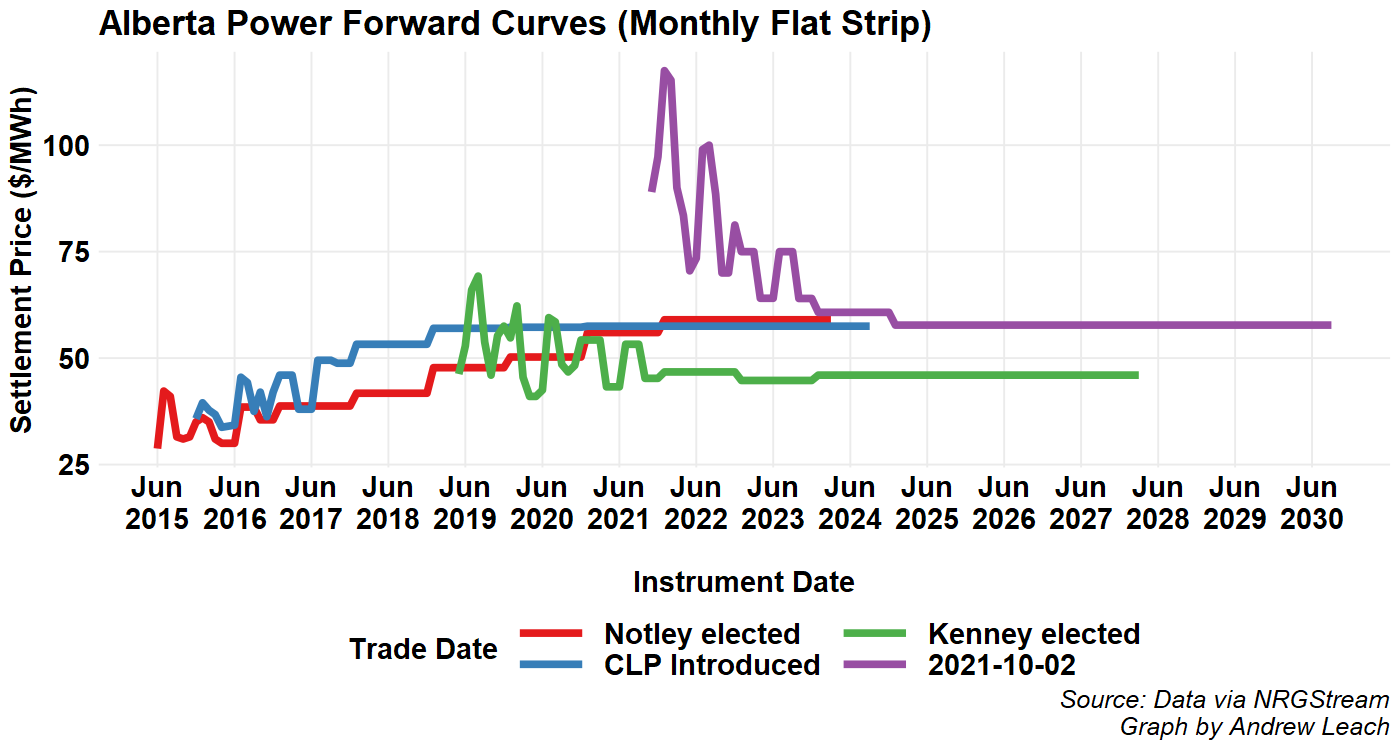
\includegraphics[width=.9\paperwidth]{../images/forwards_kenney.png}}; \vspace{1cm}
   \vfill
\end{frame}



\begin{frame}{Forward Markets}
   \tikz [remember picture,overlay]
    \node[yshift=-.5cm,xshift=0cm] at (current page.center)
        {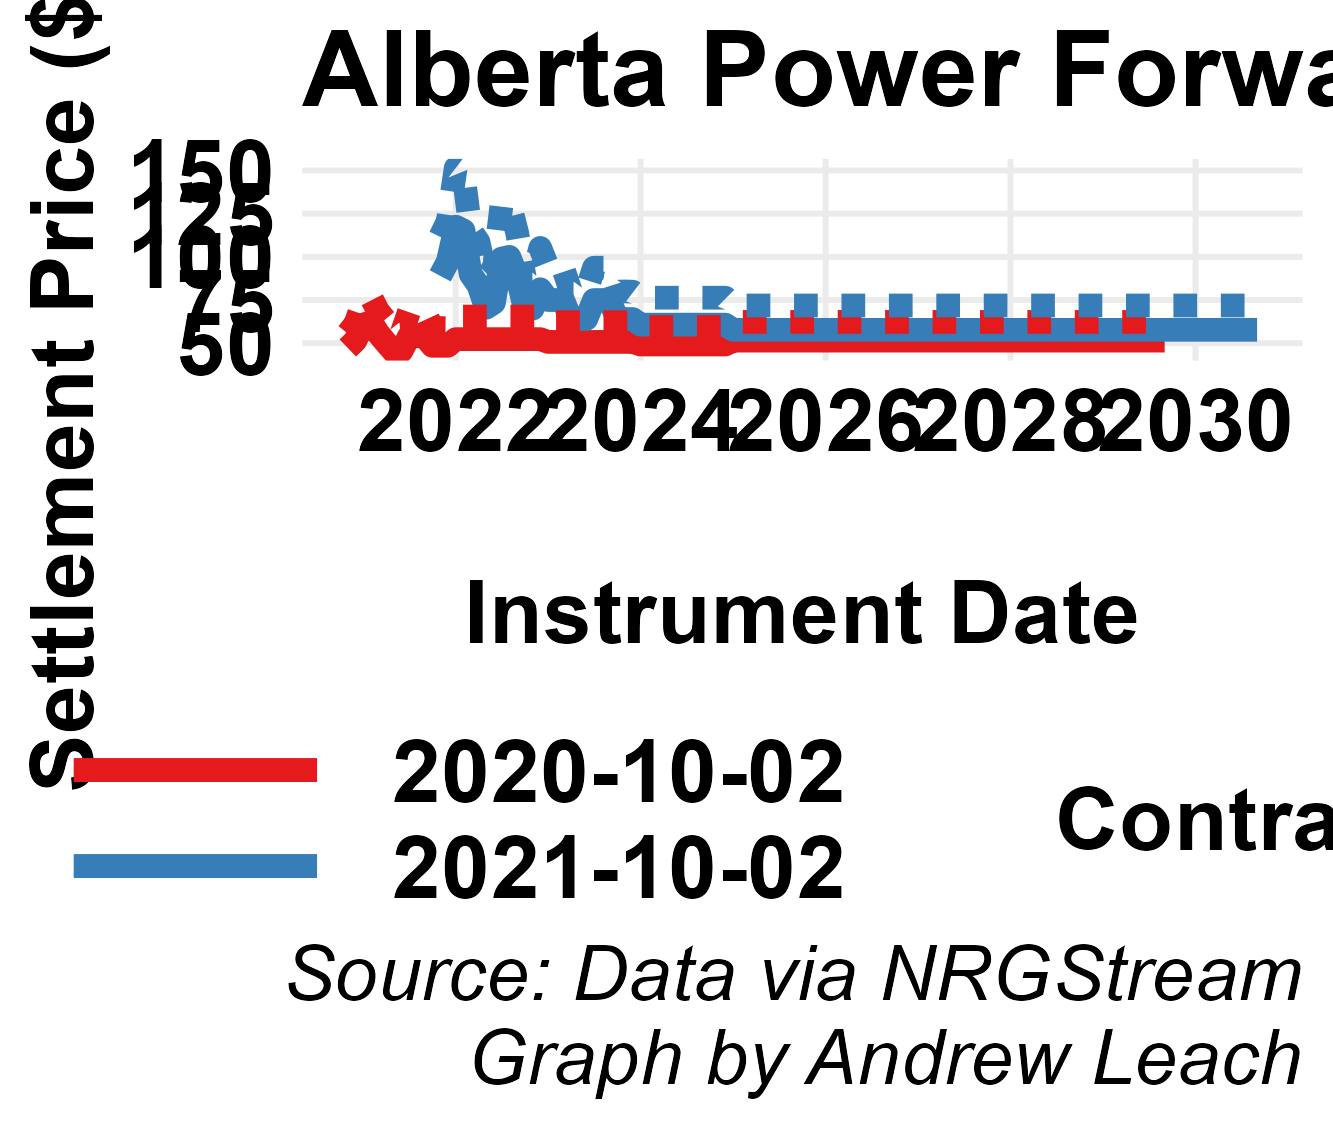
\includegraphics[width=.9\paperwidth]{../images/forwards.png}}; \vspace{1cm}
   \vfill
\end{frame}


\begin{frame}{Forward Markets}
   \tikz [remember picture,overlay]
    \node[yshift=-.5cm,xshift=0cm] at (current page.center)
        {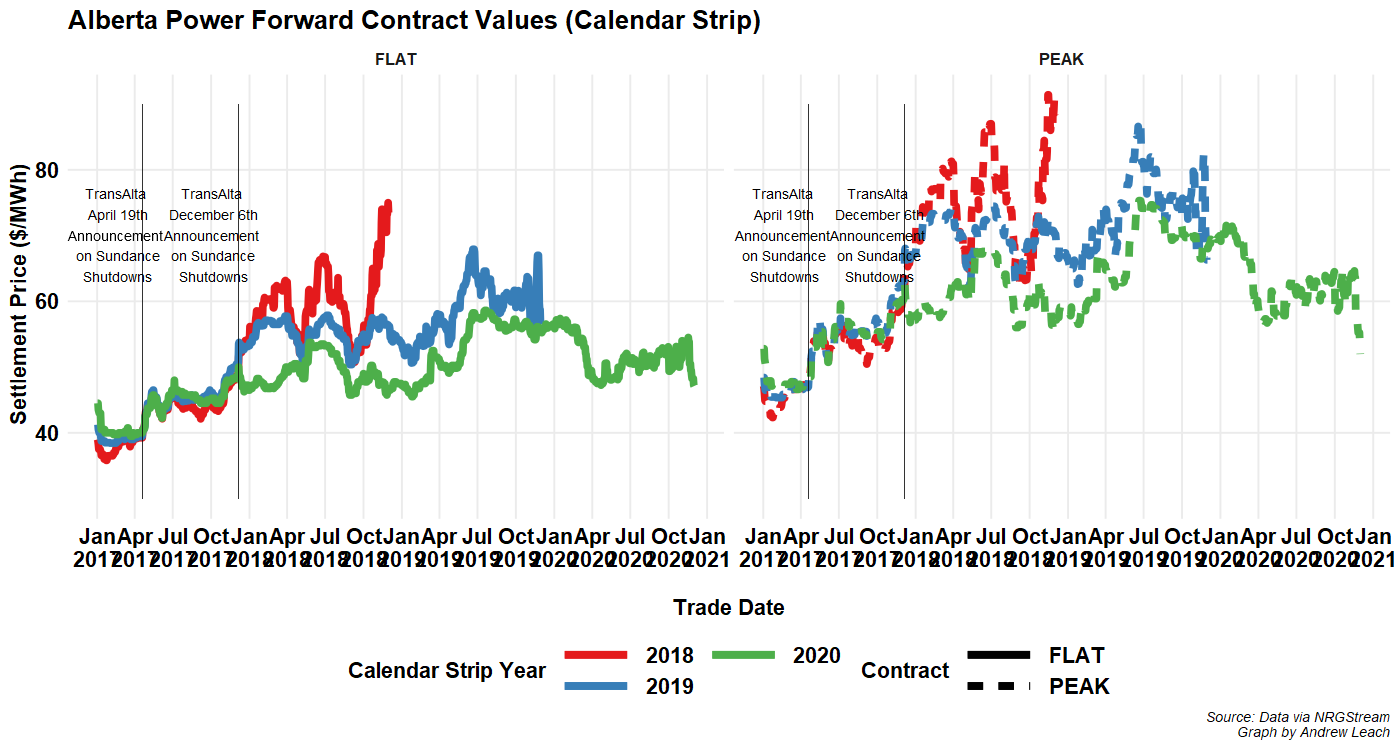
\includegraphics[width=.9\paperwidth]{../images/forwards_2017.png}}; \vspace{1cm}
   \vfill
\end{frame}





\begin{frame}{Forward Markets}
   \tikz [remember picture,overlay]
    \node[yshift=-.5cm,xshift=0cm] at (current page.center)
        {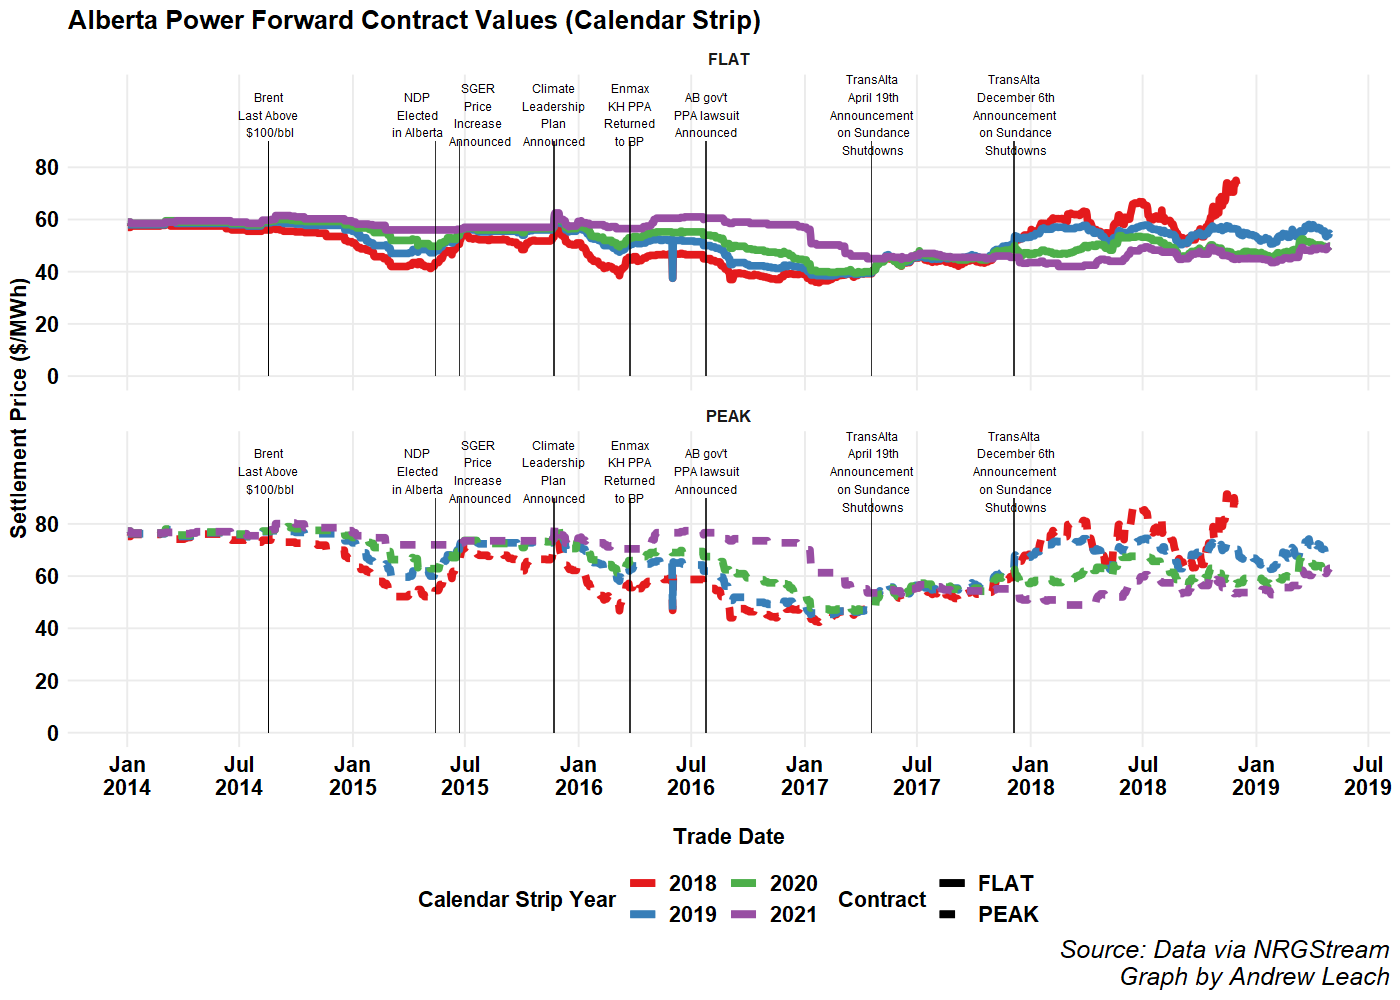
\includegraphics[width=.9\paperwidth]{../images/forwards_long.png}}; \vspace{1cm}
   \vfill
\end{frame}

\section{PPAs}

\begin{frame}{The Balancing Pool: What on earth does it do?}
\vspace{-.2cm}\centering
\hspace{-1.5cm}\begin{tabular}{p{1.1\linewidth}}
    \centering
    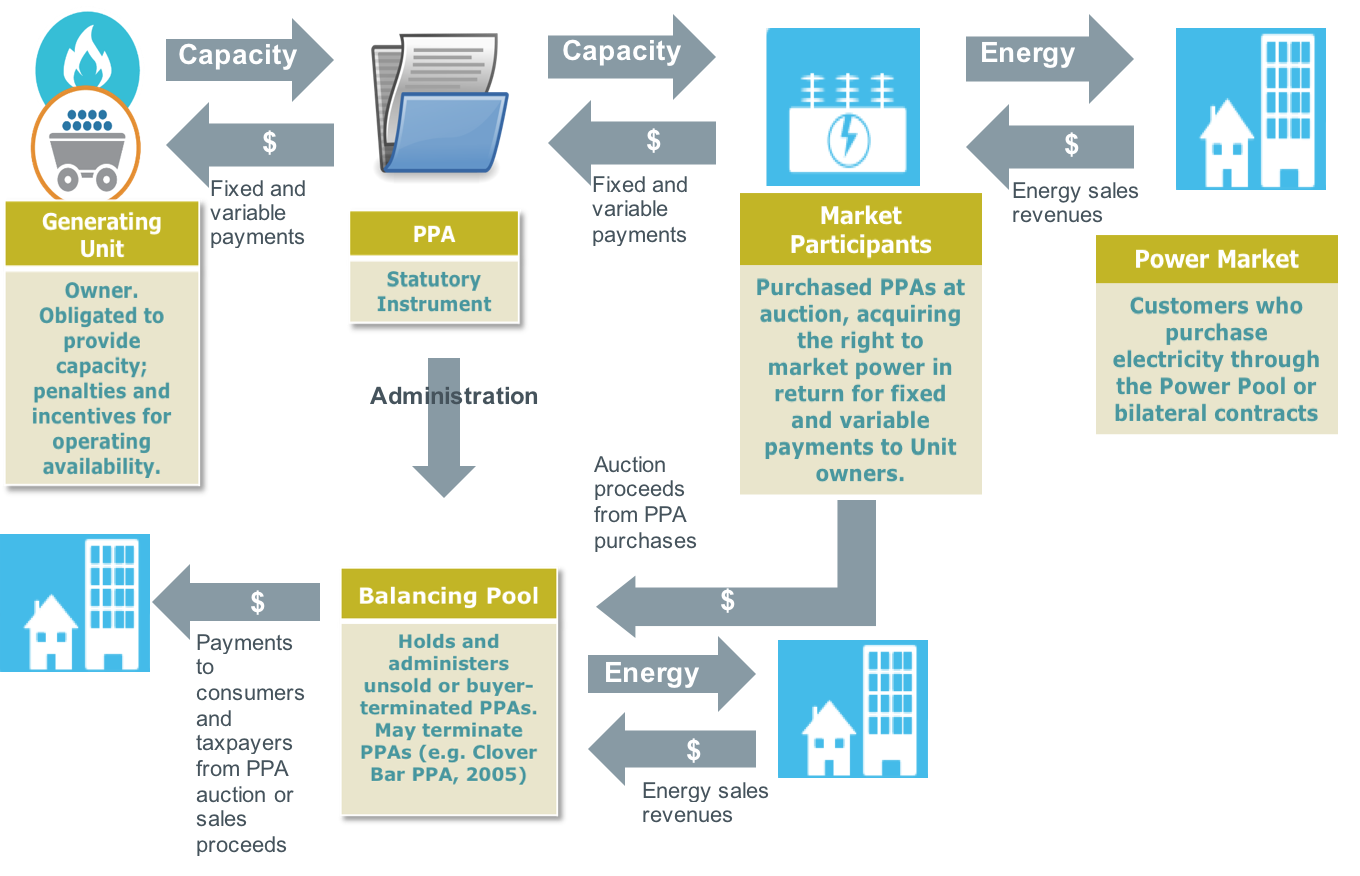
\includegraphics[width=.9\linewidth]{../images/balancingpool.png} \\[\abovecaptionskip]
  Source: Capital Power
\end{tabular}

\vfill \end{frame}



\section{Alberta Market Evolution}

\begin{frame}{Alberta's Evolving Electricity Market}
\begin{itemize}
\setlength\itemsep{2em}
\item Capacity Market
\item Coal Phase Out
\item Renewables (the REP Program)
\item Carbon Pricing
\end{itemize}

\vfill \end{frame}


\begin{frame}{Costs of New Capacity Additions}
   \tikz [remember picture,overlay]
    \node[yshift=-.25cm,xshift=0cm] at (current page.center)
        {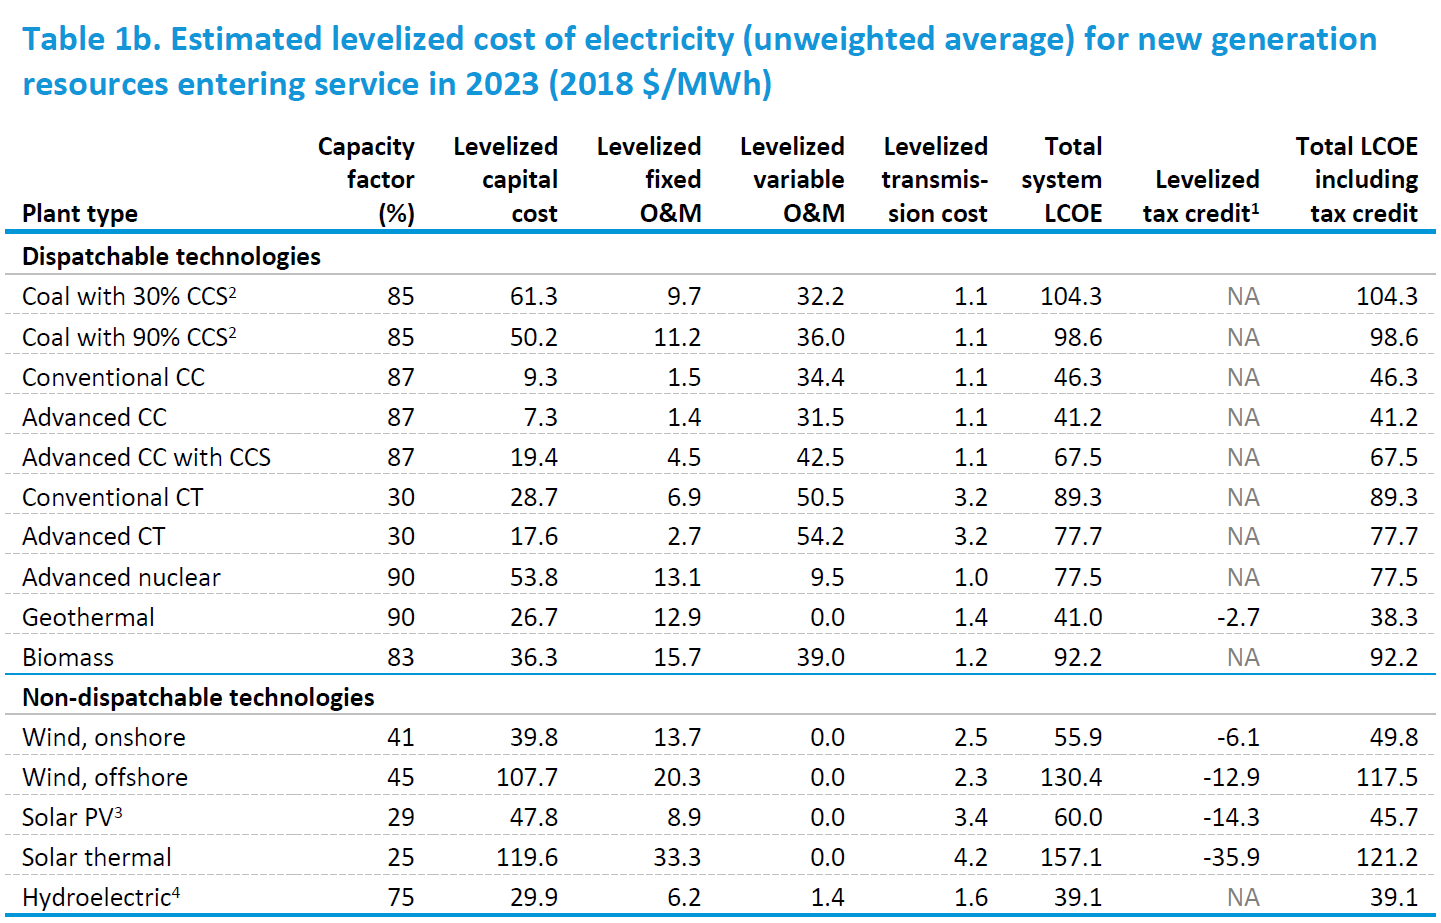
\includegraphics[width=.9\paperwidth]{../images/eia_lcoe_2019_avg.png}}; \vspace{1cm}
   \\[\abovecaptionskip]  \vspace{5.5cm}
   \tiny{See for more information: \url{https://www.lazard.com/media/451086/lazards-levelized-cost-of-energy-version-130-vf.pdf}}
   \vfill
\end{frame}



\begin{frame}{Price Capture by Technology}
   \tikz [remember picture,overlay]
    \node[yshift=-.5cm,xshift=0cm] at (current page.center)
        {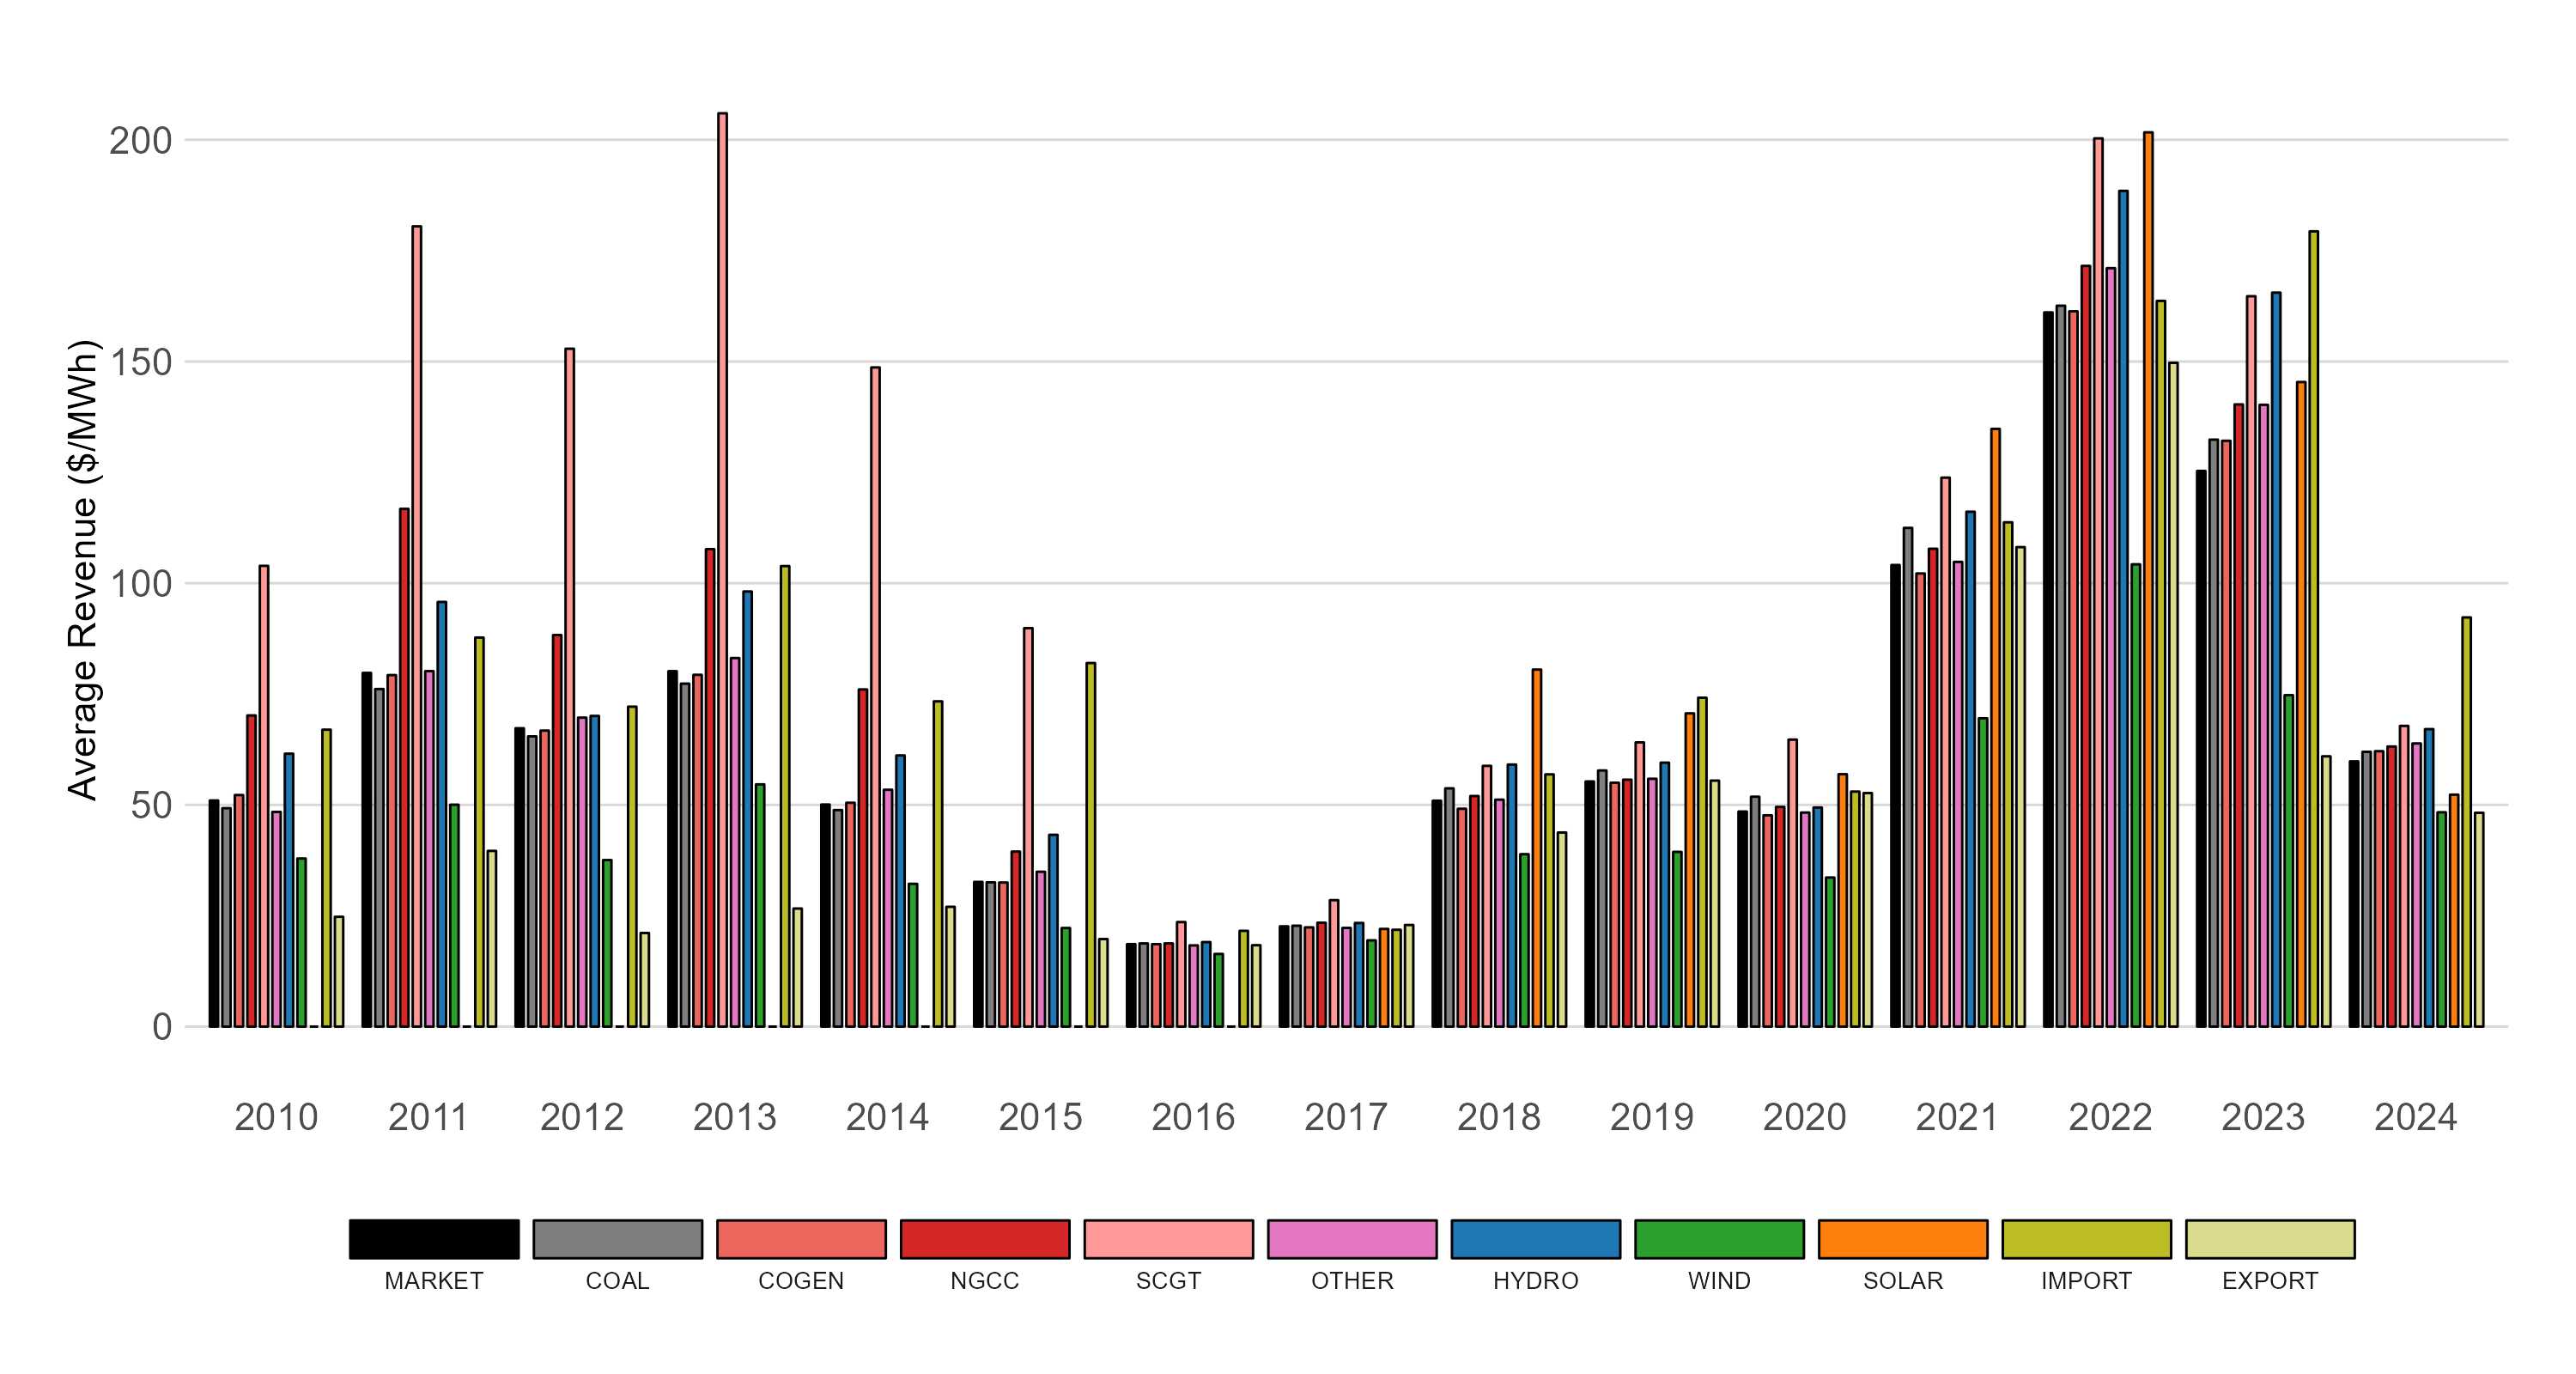
\includegraphics[width=.9\paperwidth]{../images/price_capture.png}}; \vspace{1cm}
   \vfill
\end{frame}



\begin{frame}{Price Capture by Technology}
   \tikz [remember picture,overlay]
    \node[yshift=-.5cm,xshift=0cm] at (current page.center)
        {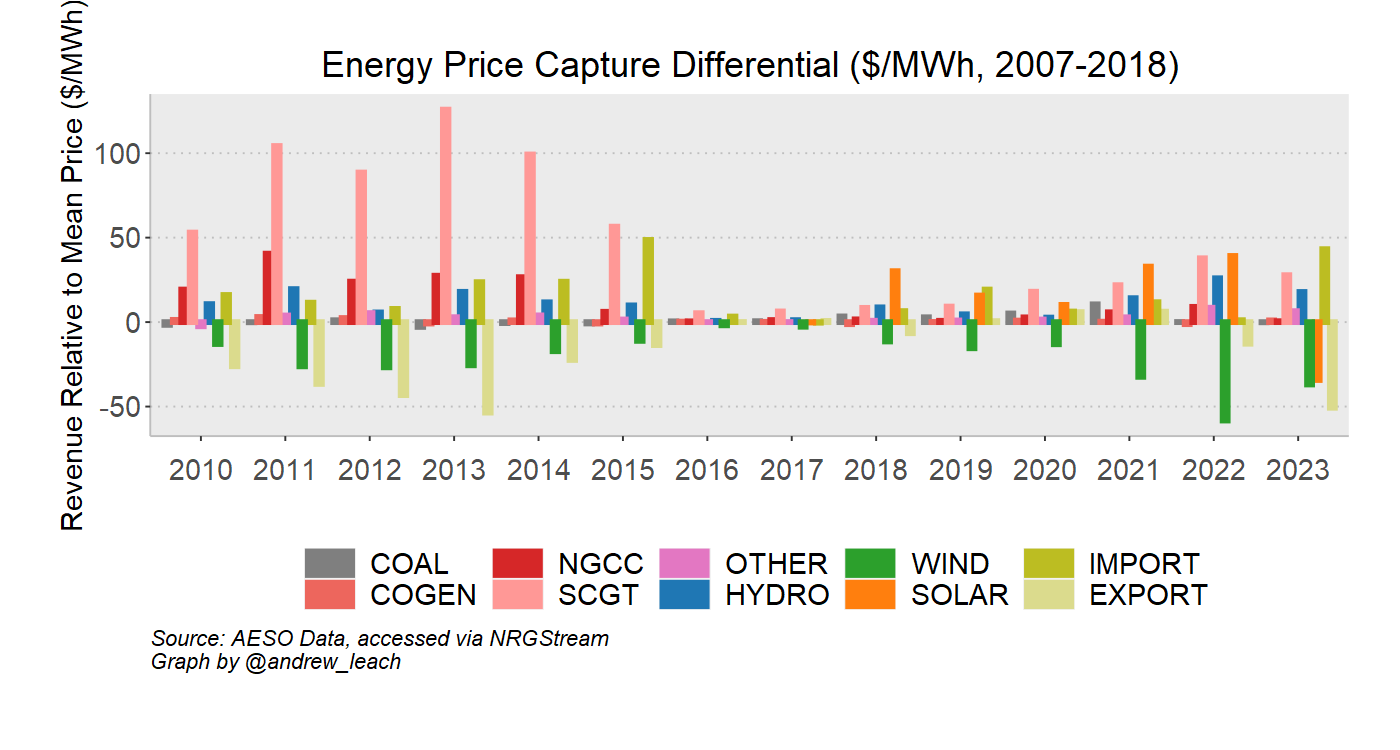
\includegraphics[width=.9\paperwidth]{../images/price_capture_avg.png}}; \vspace{1cm}
   \vfill
\end{frame}

\begin{frame}{Evolution of Technology}
   \tikz [remember picture,overlay]
    \node[yshift=-.5cm,xshift=0cm] at (current page.center)
        {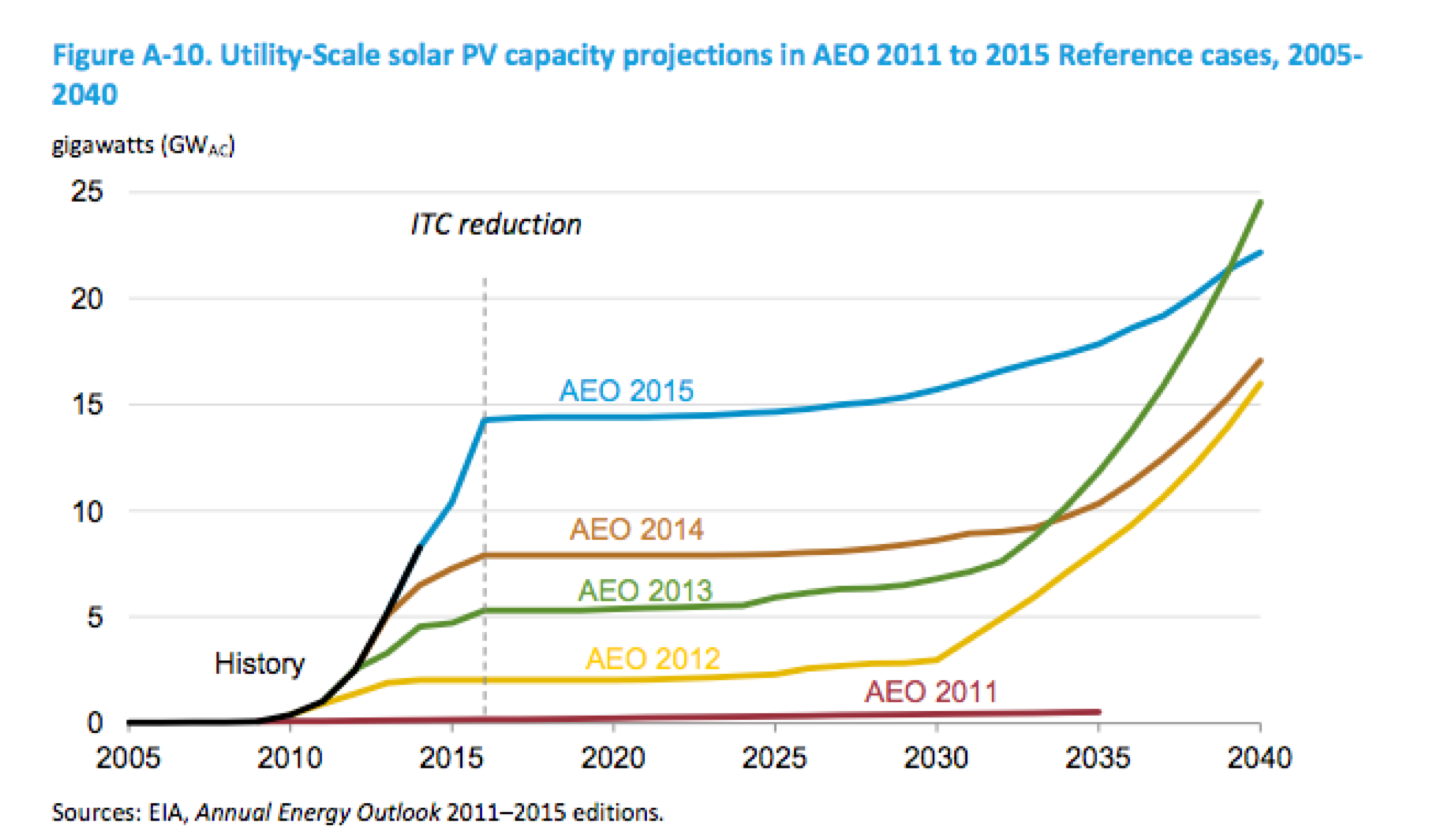
\includegraphics[width=.9\paperwidth]{../images/eia_aeo_solar.png}}; \vspace{1cm}
   \vfill
\end{frame}

\begin{frame}{Evolution of Technology}
   \tikz [remember picture,overlay]
    \node[yshift=-.5cm,xshift=0cm] at (current page.center)
        {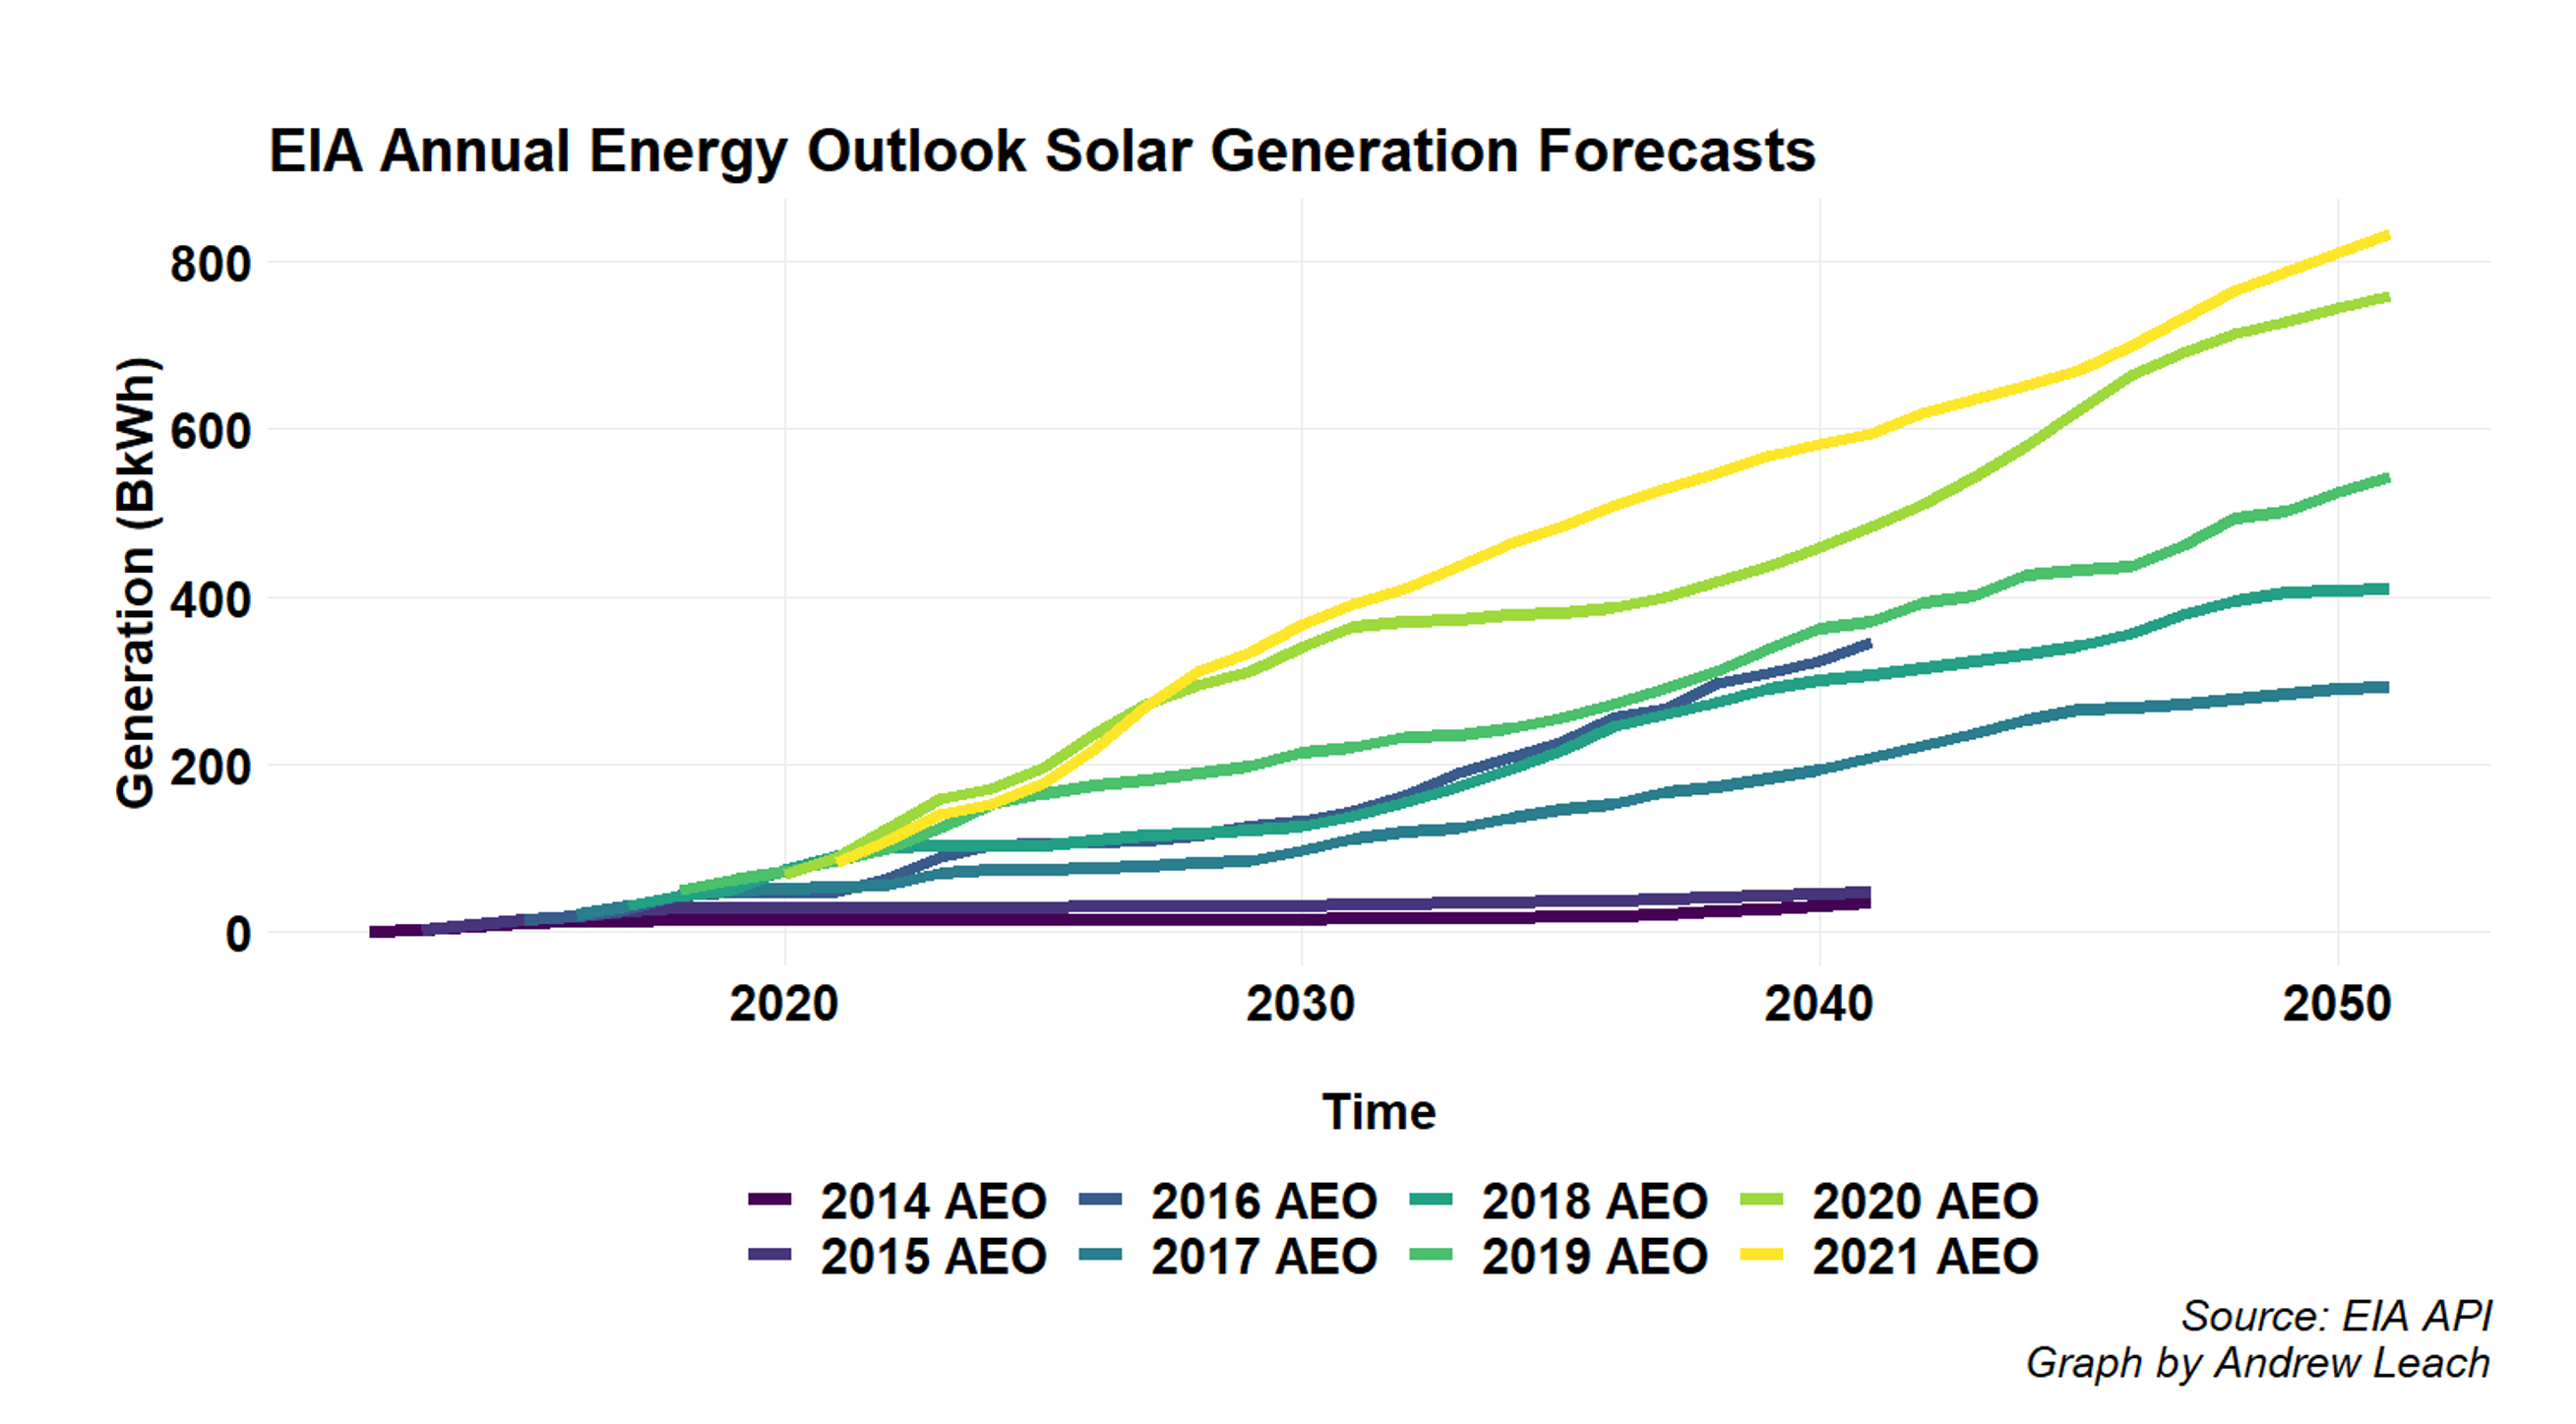
\includegraphics[width=.9\paperwidth]{../images/solar_eia.png}}; \vspace{1cm}
   \vfill
\end{frame}


\begin{frame}{Evolution of Technology}
   \tikz [remember picture,overlay]
    \node[yshift=-.5cm,xshift=0cm] at (current page.center)
        {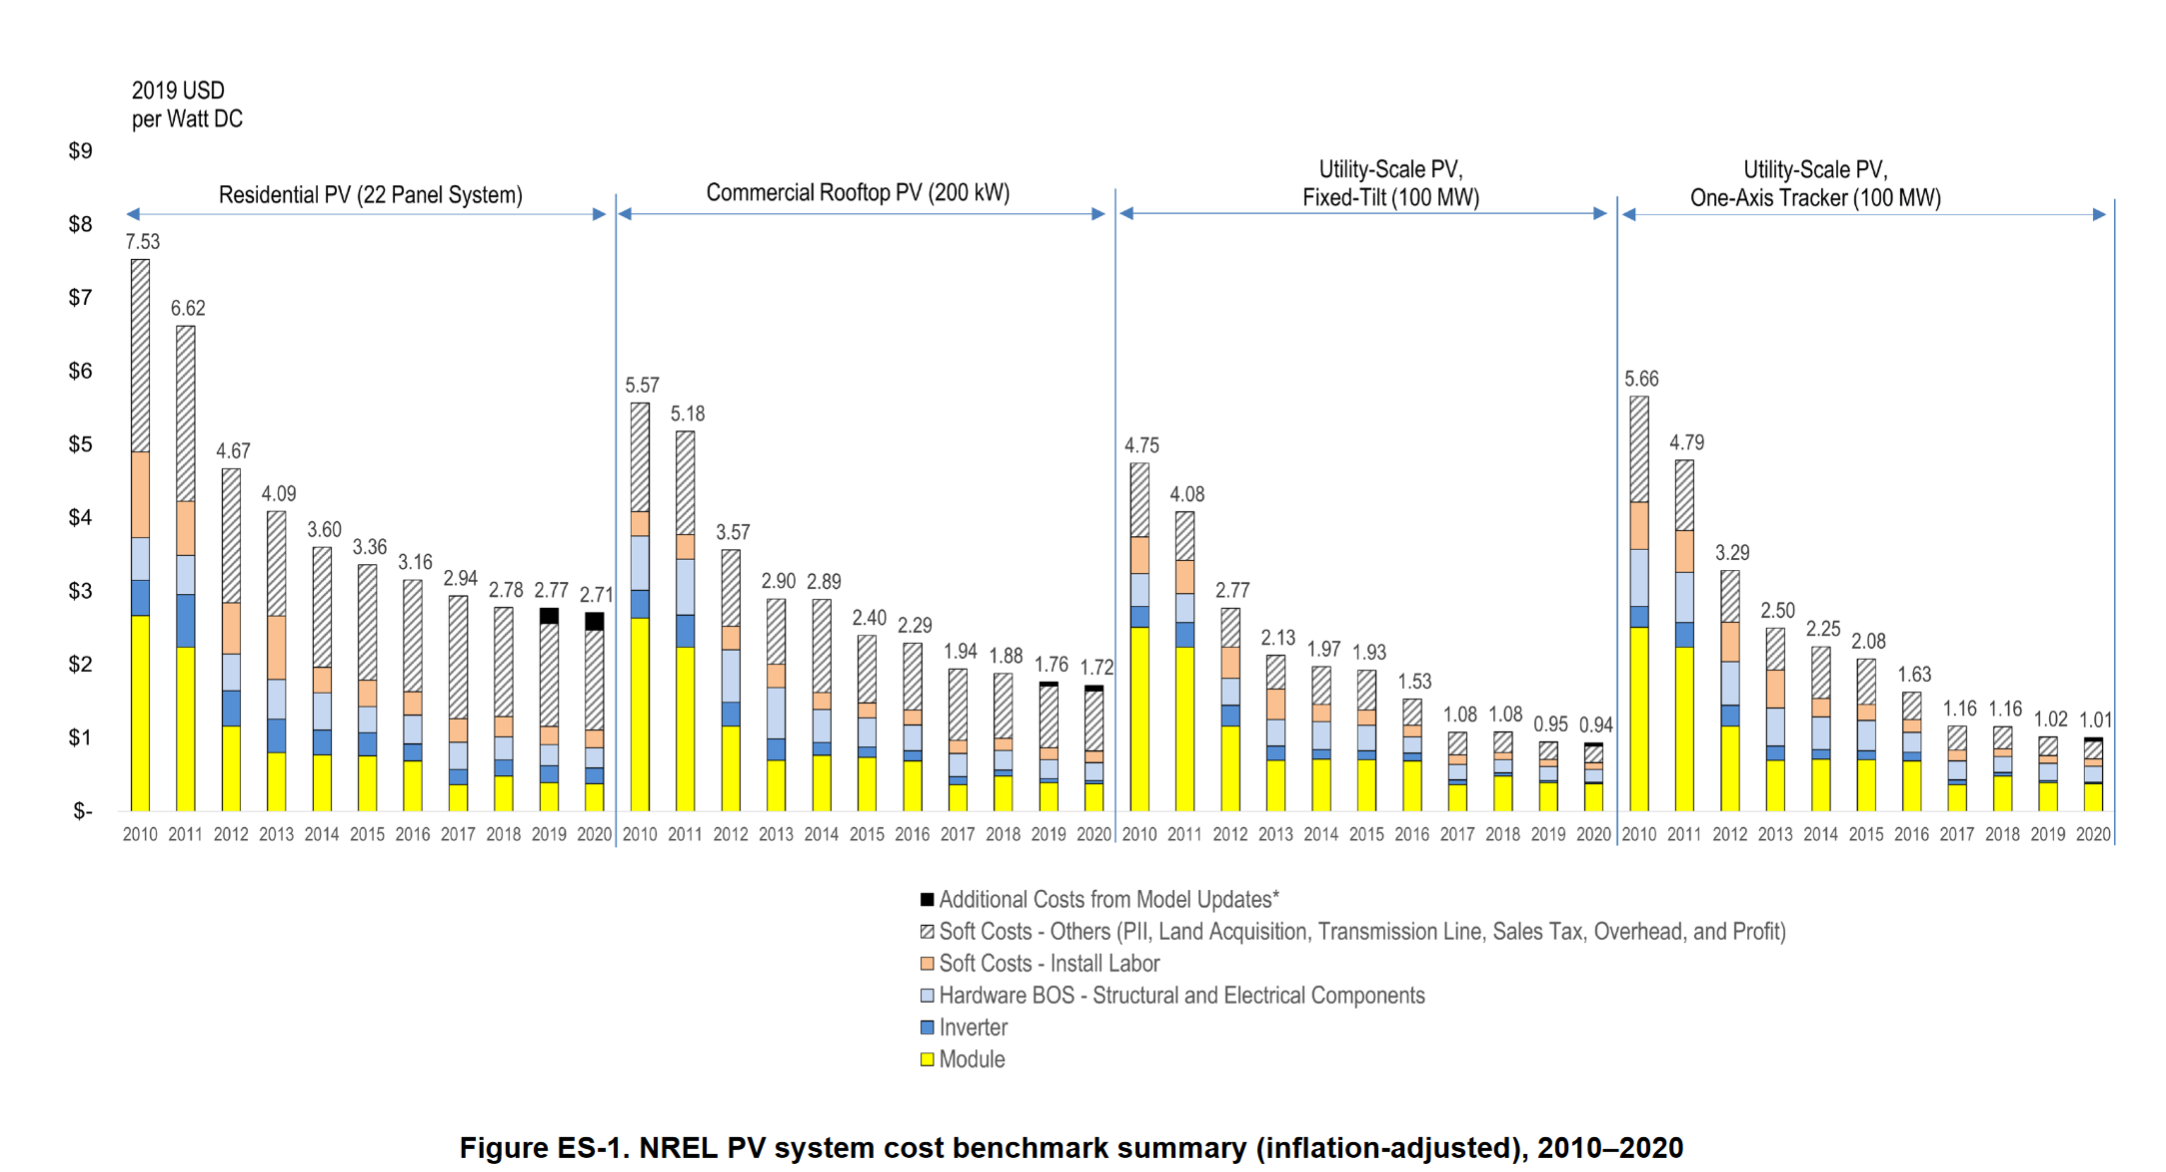
\includegraphics[width=.9\paperwidth]{../images/solar_costs.png}}; \vspace{1cm}
   \vfill
   \vspace{4cm}\tiny{Source: NREL}  \hfill
\end{frame}




\begin{frame}{GHG Policy and Electricity Supply}
   \tikz [remember picture,overlay]
    \node[yshift=-.5cm,xshift=0cm] at (current page.center)
        {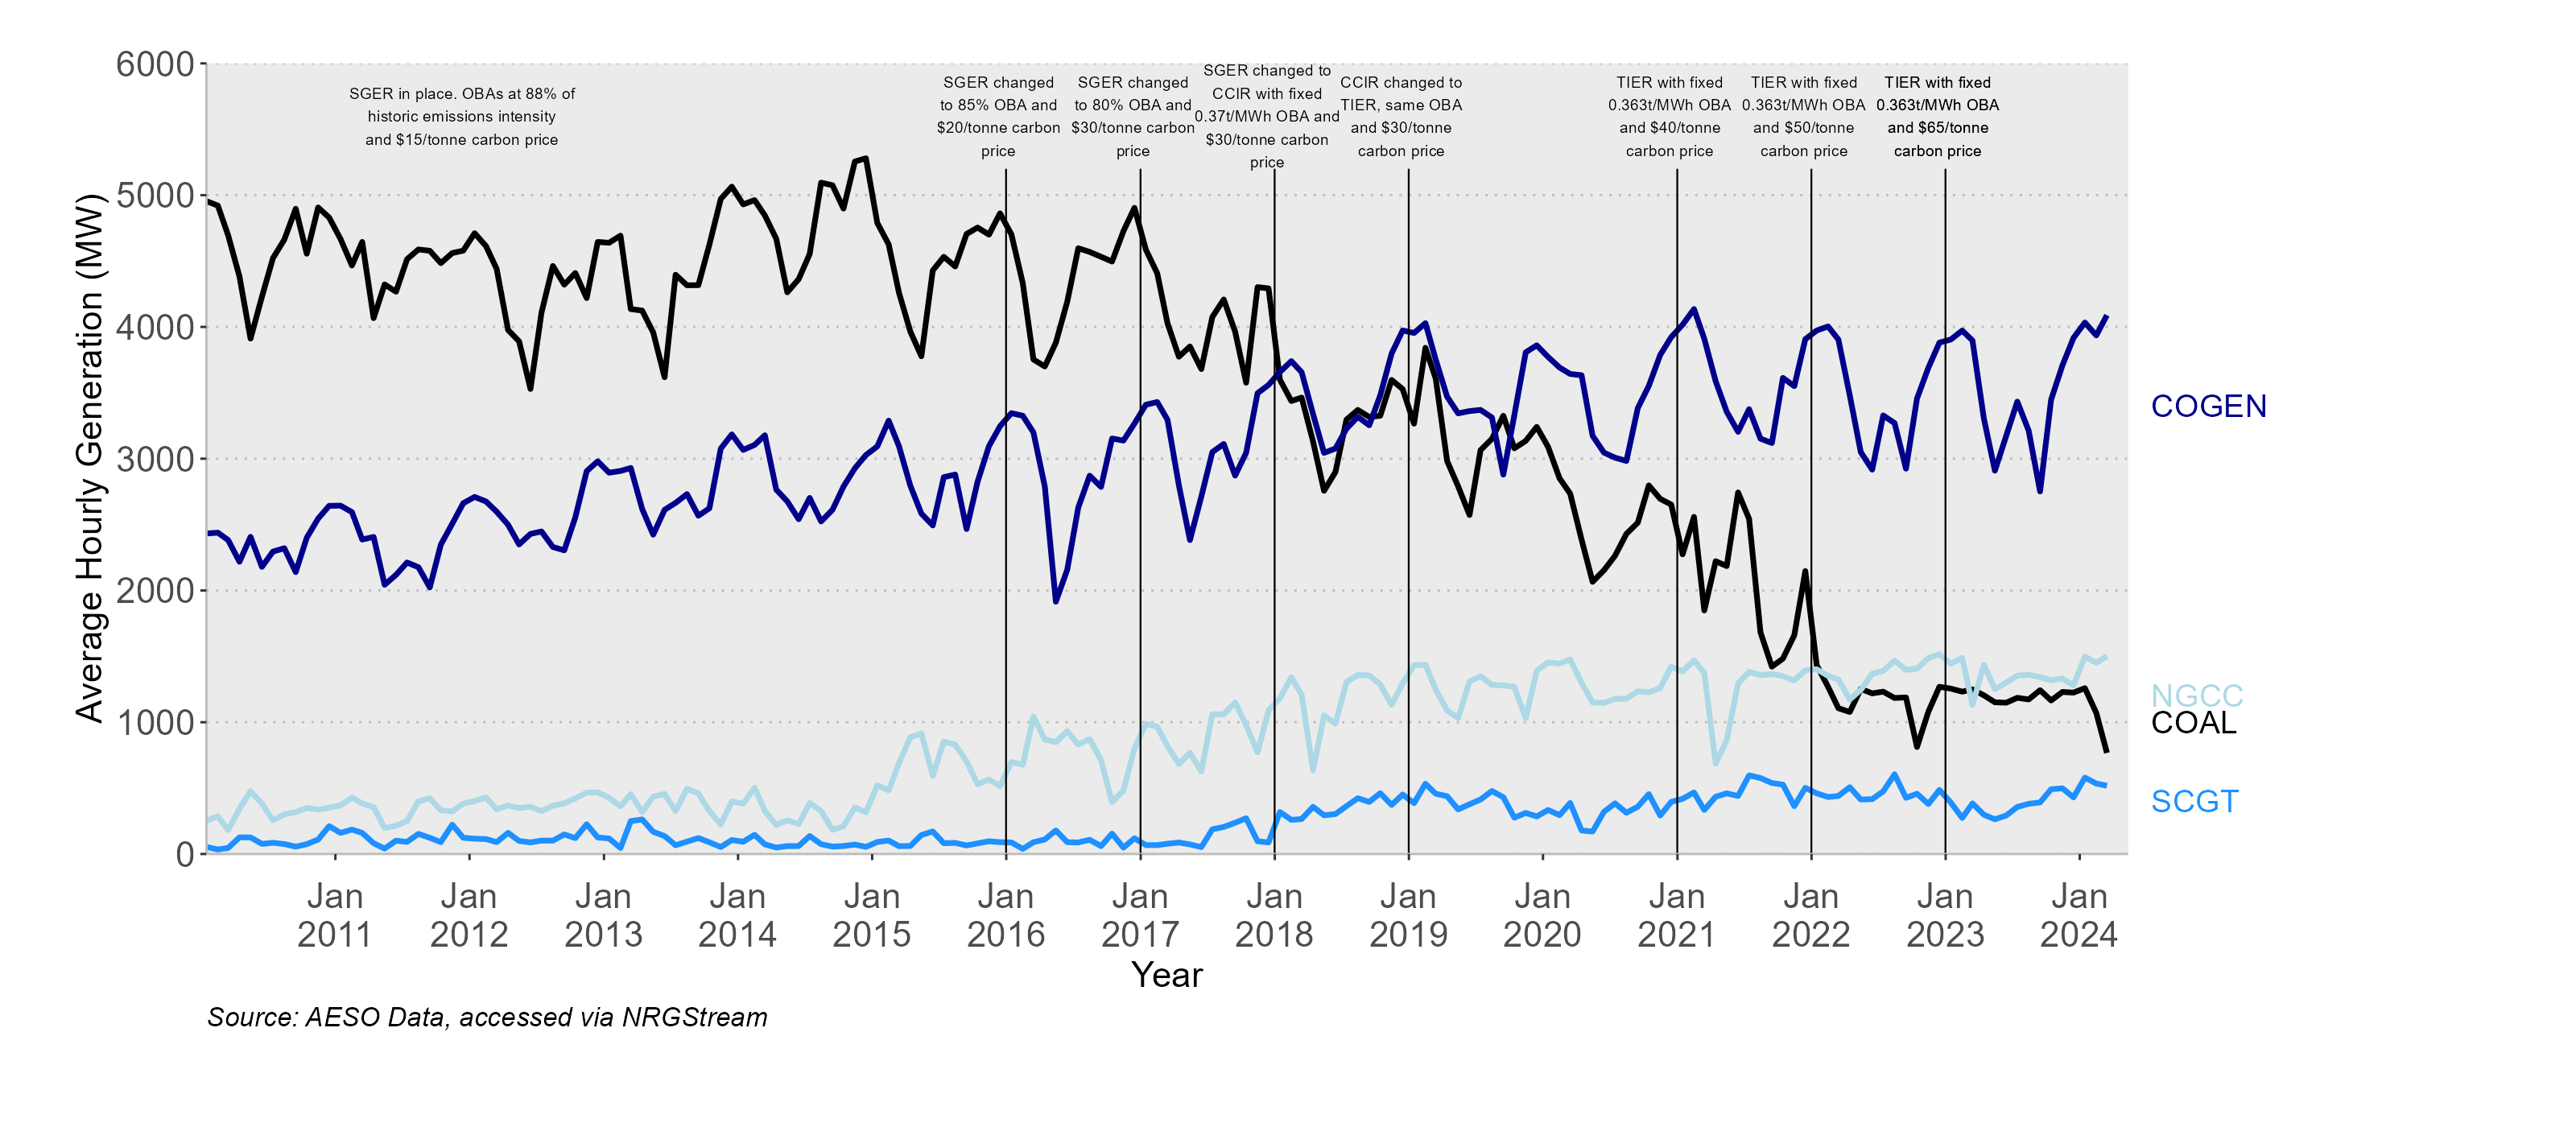
\includegraphics[width=.95\paperwidth]{../images/gen_ghg_price.png}}; \vspace{1cm}
   \vfill
\end{frame}



\begin{frame}{GHG Policy and Electricity Supply}
   \tikz [remember picture,overlay]
    \node[yshift=-.5cm,xshift=0cm] at (current page.center)
        {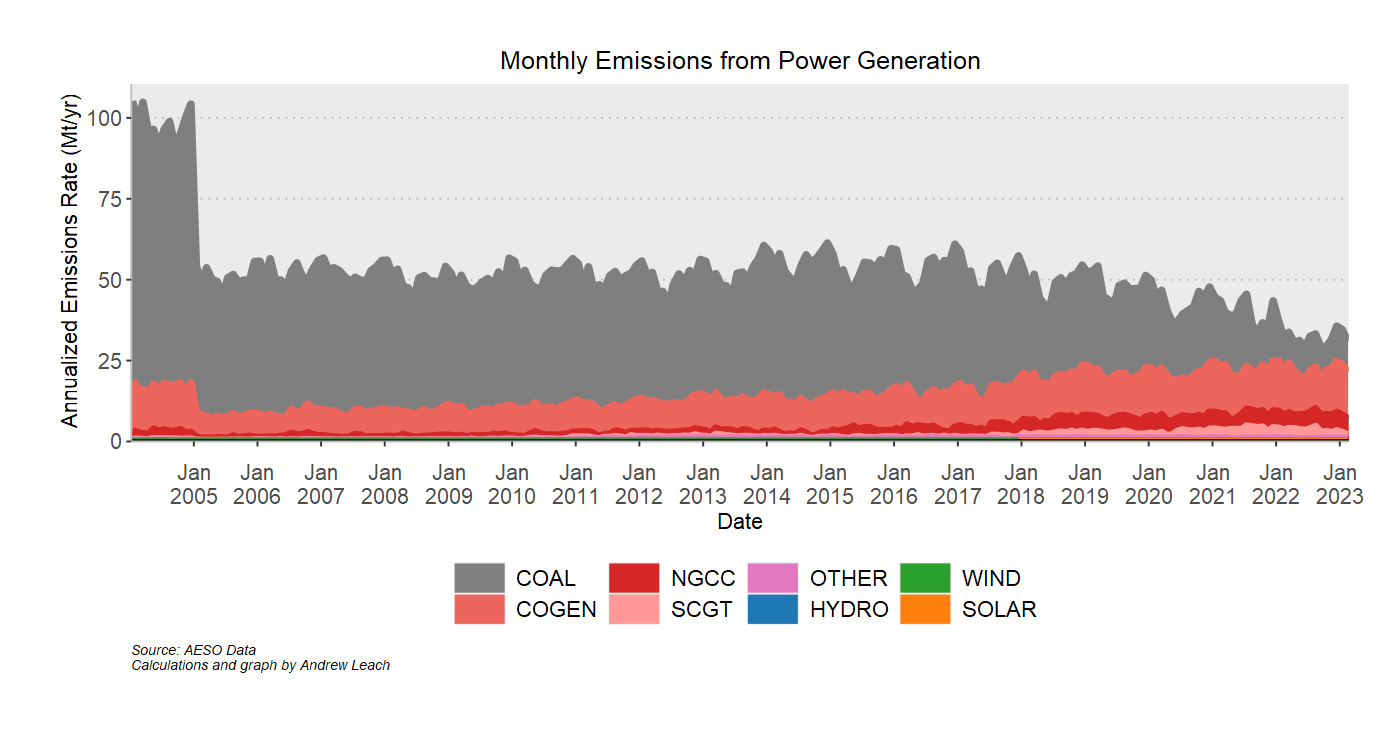
\includegraphics[width=.95\paperwidth]{../images/monthly_ghgs.png}}; \vspace{1cm}
   \vfill
\end{frame}


\begin{frame}{GHG Policy and Electricity Supply}
   \tikz [remember picture,overlay]
    \node[yshift=-.5cm,xshift=0cm] at (current page.center)
        {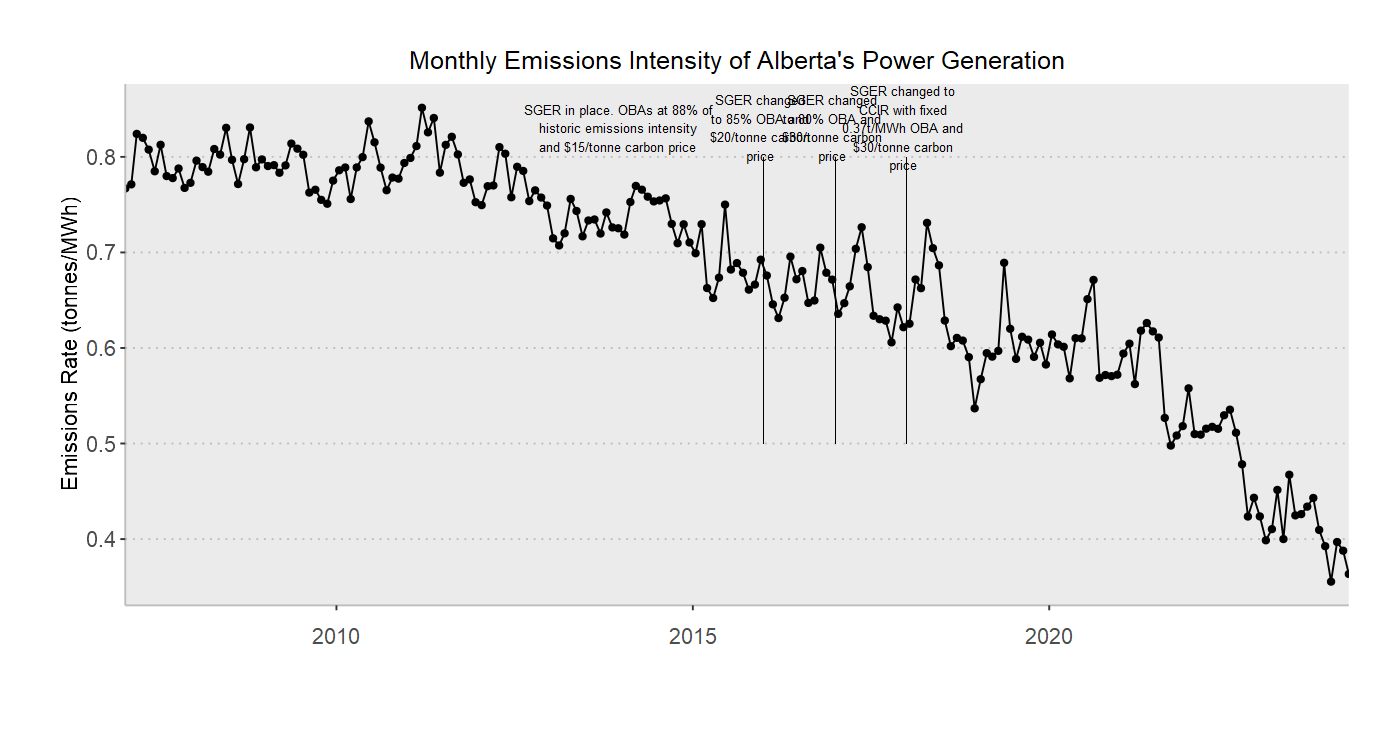
\includegraphics[width=.95\paperwidth]{../images/monthly_ghg_mwh.png}}; \vspace{1cm}
   \vfill
\end{frame}


%\begin{frame}{GHG Emissions from Electricity}
%   \tikz [remember picture,overlay]
%    \node[yshift=-.5cm,xshift=0cm] at (current page.center)
%        {\includegraphics[width=.8\paperwidth]{../inventory_ghg_mwh.png}}; \vspace{1cm}
%   \vfill
%\end{frame}



%\begin{frame}{GHG Emissions from Electricity}
%   \tikz [remember picture,overlay]
%    \node[yshift=-.5cm,xshift=0cm] at (current page.center)
%        {\includegraphics[width=.8\paperwidth]{../elec_share.png}}; \vspace{1cm}
%   \vfill
%\end{frame}



\end{document}
